\chapter{Data entry in an office setting}\label{ch:Study1}
\begin{mynote}
\subsubsection{Chapter outline}

In this chapter I describe an explorative interview study and a contextual inquiry study on understanding data entry in a naturalistic office setting.
The interview study revealed that a major aspect of data entry work in this setting is collecting information from multiple sources with different levels of access, which then became the focus of the rest of the thesis. The contextual interview study showed office workers regularly interrupt themselves as soon as they realise they need digital information, but barely interrupt themselves to access paper sources as there is effort involved. Digital interruptions took longer than intended as participants were distracted by task-irrelevant information.

\end{mynote}

\section{Study 1: Understanding data entry work in a financial office}\label{ch:Study1}
 
\subsection{Introduction}
As data entry is a common task and it is important this is done both accurately and efficiently, work has been done to design and optimise data entry interfaces to support fast and accurate data entry \citep[e.g.][]{Oladimeji2013, Vertanen2015, Wiseman2013a}.
However, it is not just the input method that determines efficiency and accuracy but also other aspects of the task, such as the environment within which it is conducted \citep{Payne2013, Randall2014}.

\citet{Evans2012} looked if people's text entry and mouse pointing behaviour in a lab setting was comparable to how they would normally perform these inputting tasks in their everyday life. They remotely observed people's input behaviour on their personal computer, and compared this with their performance on similar tasks in a lab. Participants installed a tool on their personal computer which logged all text entry and mouse pointing behaviour they performed in one workweek. Examples of tasks that were carried out were sending personal messages to friends and browsing the web. There were no differences in uncorrected errors or text entry speed between the lab and the field, but they did find that participants corrected more errors in the lab. This study shows that people check and correct their entries more when they are in a controlled environment and are focused on the task, though the measured behaviour on people's personal computers mostly included tasks where accuracy may not have been considered important, such as sending an informal chat message to a friend. 

In order to support people in their data entry work, it is important to first have a better understanding of the types of data entry tasks they have to conduct, and the physical environment in which this is done. Therefore, the first study of this thesis is an explorative study. I visited and interviewed people who conduct data entry tasks as part of their daily work in the finance departments of two universities. This user group was chosen as they have a lot of data entry tasks as part of their job, and it is an area where it is important to enter data accurately, but there is also time pressure to finish work on time. Furthermore, it was an accessible user group to approach for the researcher.

Previous research has given us a good understanding of which factors may influence people's performance on a data entry task. The current study aims to study how these factors are laid out in an applied setting. Furthermore, this study gives an opportunity to see if there are additional problems that influence data entry performance, that are currently not acknowledged in existing literature. 

\subsection{Method}
\subsubsection{Participants}
Nine participants (four male) took part in the study. They were employees from two public universities and their work involved receiving various requests for payment, checking the information of these requests was correct, and entering the information along with administration data into computer systems. Ages ranged from 18 to 52 (two participants wished to not disclose their age). Their level of experience differed, with some participants having just started doing this type of job and other participants working in Finance for 17 years. All but one worked full-time. Table \ref{table:ch3_participants} shows further demographic details of the participants. Typical tasks participants dealt with were checking and entering expense forms sent by staff and students, paying salaries and pensions, controlling research budgets, monitoring university income and expenses and entering employee information. Participants were recruited by sending invitations to opt-in mailing lists of Finance departments, and were reimbursed with a \pounds10 Amazon voucher.

\begin{table}
\caption{Participant information.}
\centering
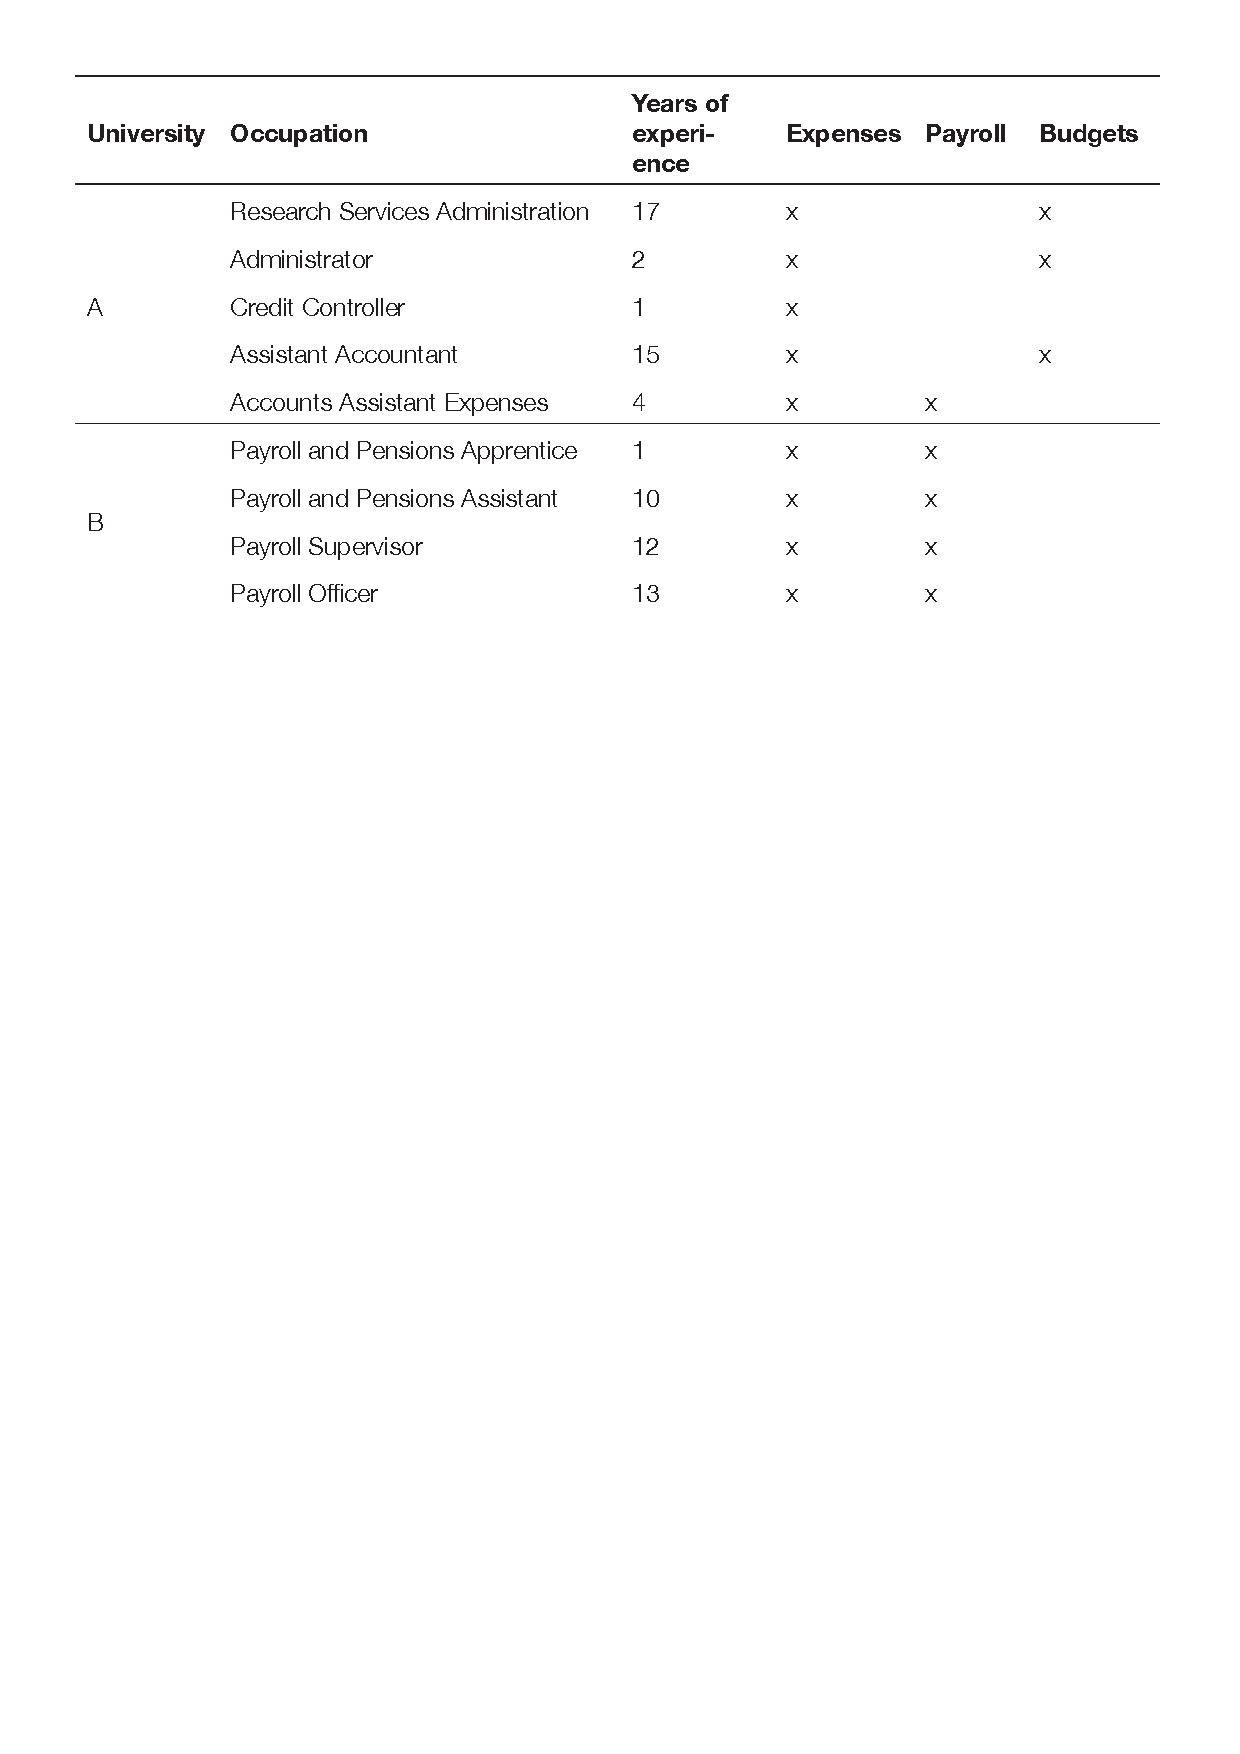
\includegraphics[width=0.9\textwidth]{images/ch12/Study1-Table1.pdf}
\vspace{-3pt}
\label{tbl:ch12-Table1}
\end{table}

\begin{comment}
\begin{table}[htp]
\centering
\resizebox{\textwidth}{!}{%
\begin{tabular}{llllllll}
{\bf ID} & {\bf Age} & {\bf Gender} & {\bf Nationality} & {\bf Occupation}                                                             & {\bf University} & {\bf \begin{tabular}[c]{@{}l@{}}Experience in\\ Finance\\ (y = years,\\ m = months)\end{tabular}} & {\bf Deals with}                                                                                     \\ \hline
P1       & 49        & M            & Danish            & \begin{tabular}[c]{@{}l@{}}Research\\ Services\\ Administration\end{tabular} & A                & 17y                                                                                               & \begin{tabular}[c]{@{}l@{}}invoices,\\ statements,\\ grants\end{tabular}                             \\
P2       & 39        & F            & British           & Administrator                                                                & A                & 2y                                                                                                & \begin{tabular}[c]{@{}l@{}}funding,\\ expenses,\\ room\\ bookings,\\ events\end{tabular}             \\
P3       & 20        & F            & British           & \begin{tabular}[c]{@{}l@{}}Credit\\ Controller\end{tabular}                  & A                & 7m                                                                                                & \begin{tabular}[c]{@{}l@{}}money that\\ comes in,\\ payments\end{tabular}                            \\
P4       & -         & M            & British           & \begin{tabular}[c]{@{}l@{}}Assistant\\ Accountant\end{tabular}               & A                & 15y                                                                                               & \begin{tabular}[c]{@{}l@{}}research\\ budgets,\\ expenses\end{tabular}                               \\
P5       & 33        & F            & British           & \begin{tabular}[c]{@{}l@{}}Accounts\\ Assistant\\ Expenses\end{tabular}      & A                & 4y2m                                                                                              & \begin{tabular}[c]{@{}l@{}}expenses,\\ employee\\ information,\\ supplier\\ information\end{tabular} \\
P6       & 18        & M            & British           & \begin{tabular}[c]{@{}l@{}}Payroll and\\ Pensions\\ Apprentice\end{tabular}  & B                & 6m                                                                                                & \begin{tabular}[c]{@{}l@{}}salaries,\\ expenses,\\ pensions\end{tabular}                             \\
P7       & 40        & F            & British           & \begin{tabular}[c]{@{}l@{}}Payroll and\\ Pensions\\ Assistant\end{tabular}   & B                & 10y                                                                                               & \begin{tabular}[c]{@{}l@{}}salaries,\\ expenses,\\ pensions\end{tabular}                             \\
P8       & 52        & M            & British           & \begin{tabular}[c]{@{}l@{}}Payroll\\ Supervisor\end{tabular}                 & B                & 12y                                                                                               & \begin{tabular}[c]{@{}l@{}}salaries,\\ expenses,\\ pensions\end{tabular}                             \\
P9       & -         & F            & British           & Payroll Officer                                                              & B                & 13y                                                                                               & \begin{tabular}[c]{@{}l@{}}salaries,\\ expenses,\\ pensions,\\ employee \\ information\end{tabular} 
\end{tabular}
}
\caption[Study 1 participant information]{Participant information.}
\label{table:ch3_participants}
\end{table}
\end{comment}

\subsubsection{Materials}
Materials that were used during the interview were a voice recorder, a paper copy of an interview script with the interview topics and guiding questions, a consent form, an information sheet for the participant and a notebook and pen to make notes. The interview script, information sheet and consent form are included in the Appendix. 
Each interview covered four guiding topics, which are briefly described in Table \ref{table:ch3_interviewtopics}. For each topic, a number of questions were written out beforehand. These questions were used as a starting point to get the participant talking and guide the interview. Based on what the participant was saying follow-up questions were asked. The audio transcription program ExpressScribe was used to transcribe the interviews. The data analysis programs Nvivo and Atlas.ti were used to analyse the data. Nvivo was used to code the interview transcripts and notes. Atlas.ti was used to complement the analysis in Nvivo and allowed to identify relations between codes.

\begin{table}[htp]
\centering
    \begin{tabular}{ | l | p{10cm} |}
    \hline
     Topic & Description \\ \hline
    Job description & A description of the tasks that the interviewee deals with. The purpose of this topic was to start the interview easy and give the interviewee the opportunity to explain what their job entails. \\ \hline
    Number transcription & This includes questions on when and how people typically enter numbers for work.  \\ \hline
Environment & This topic includes people's physical work environment, and the organisation they are a part of. \\ \hline
Demonstration &  Interviewees were asked to give a demonstration of entering data into their system. The aim of this part of the interview is to see the type of data entry tasks people have to do, and also gives a chance to see the information sources and systems people currently use. \\
    \hline
    \end{tabular}
    \caption[Study 1 interview topics]{Interview topics.}
    \label{table:ch3_interviewtopics}
\end{table}%

\subsubsection{Data recording}
A voice recorder was used to audio record the interviews. One participant wished to not be audio recorded and one interview could not be audio recorded due to technical issues, so for these two interviews notes were taken of the answers. For the remaining seven interviews, notes were only made of observations and not the participants' answers. Notes were made with pen and paper. Photographs were made of the work environment and screenshots of the systems that the interviewees used.

\subsubsection{Interviewing procedure}
The interviews took place at the participants' workplace. For two interviews, the interviewee's office place was not suitable for talking so the interview took place in a common room nearby, and these participants showed their workplace and completed a demonstration of entering data after the interview. 
Participants were welcomed and informed about the study. They received a paper information sheet with the outline of the study and contact details of the researcher to keep for future reference. They were also asked to read and sign a consent form.

The interviews were semi-structured and took between 20 and 55 minutes. Each interview was reviewed afterwards, and findings sometimes fed into new questions being included or some questions being adapted in subsequent interviews.

\subsubsection{Pilot interview}
A pilot interview was conducted with an acquaintance of the researcher who worked in Finance, to test out the set-up of the study and questions. The interview took place at the participant's home, notes were taken with pen and paper, and the interview was audio-recorded using iMovie on a Macbook Pro. 

Taking notes slowed down the flow of the interview: sometimes the interviewee stopped talking to give the interviewer the opportunity to finish taking notes. Furthermore, taking notes took attention away from what the interviewee was explaining: assumptions made during the interview did not seem to be accurate in later analysis. Therefore, it was decided that note taking would be kept to a minimum. Notes would only be made of observations that could not be taken from audio recordings.

The interviewee talked elaborately about manually converting different currencies, and identified this task as the main place where errors occurred. Therefore, questions were included about if interviewees dealt with foreign currencies and converting these. 

\subsubsection{Ethical considerations}
The study was undertaken with ethical approval from the UCL Research Ethics Committee [Project ID Number UCLIC/1415/001/Staff Brumby/Borghouts]. 
At the start of each interview, participants were first informed verbally about the study. They were then given a consent form to read and sign, and were given an information sheet to keep. This information sheet contained the study information and contact details of the researcher and the project's principal researcher, should participants have any further questions after completion of the study.  They were asked permission for the interview to be audio recorded. One participant wished not to be audio recorded and notes were taken instead. 

Participants were informed that the data would be used for research purposes only and stored in accordance with the Data Protection Act 1998. They were also informed that their data would be anonymised and when used in a report or academic paper, their data would not be directly identifiable. Names of participants or the universities they were working at were not included in the interview notes and transcripts.
 
\subsection{Results}
\subsubsection{Data analysis}
After each interview or set of interviews, a first analysis took place. The audio recording was played back, notes were typed into a digital file and reviewed and the interview was transcribed verbatim. Several non-verbal cues were included in the transcription as well, such as when the interviewee laughed or sighed, as well as descriptions of when the interviewee was demonstrating something. The advantage of doing the transcription shortly after the interview was that it was still easy to remember from listening to the audio recording what was being demonstrated. Interesting findings and initial patterns that were apparent across the data were written down. 

After all interviews had been transcribed, the transcriptions and notes were printed and the data was analysed using thematic analysis \citep{Braun2006}. Anything in the data that was considered to be interesting was annotated by hand and labelled with an appropriate code. On reviewing the coding, some codes were grouped together in one code, additional codes were named, and similar codes were grouped under themes. For instance, an initial code was Notifications, such as e-mail notifications. During the second coding iteration, it was identified that people always talked about notifications in the context that they were interrupted (by a notification) rather than about notifications on its own. Therefore, notifications and interruptions were grouped into one code. 

The themes were then reviewed, to see if they addressed the purpose of the study. The transcripts and notes were then imported into Nvivo and coded digitally. Atlas.ti was used to complement this analysis and allowed to identify relations between codes. 

\subsubsection{Themes}
In total 51 codes were derived, and these were grouped into 8 main themes, which are listed and described in Table \ref{table:ch3_themes}. If codes or separate quotes did not belong in a certain theme but were still considered relevant, they were grouped in the Other category. 

\begin{table}[htp]
\centering
\resizebox{\textwidth}{!}{
    \begin{tabular}{ | p{3cm} | p{8cm} | l | l |}
    \hline
     \textbf{Theme} & \textbf{Description} & \textbf{Quotations} & \textbf{Participants} \\ \hline
     Task characteristics & People described things that were particular to their task, for instance how they structured their task, whether they switched tasks, and how long they took to complete tasks.  & 129 & 9 \\ \hline
	 Checking & People talked about checking data input as part of their job. & 103 & 9 \\ \hline 
	System & People talked about the computer system they were using to input data.  & 91 & 9 \\ \hline 
		Environment &People described their environment, for instance they talked about their physical work setting, and the work culture of their organisation. & 80 & 9 \\ \hline 
		Data &People described the data they were dealing with, for instance the type and length of data items, and from which source they copied data. & 75 & 9 \\ \hline 
		Errors &People described situations where errors were made: who made them, why were they made, what were the consequences. & 75 & 9 \\ \hline 
					 Strategy & People described the strategies they used to carry out their task.  & 54 & 9 \\ \hline 
		Importance of accuracy and paper trails &People talked about the sensitivity of financial data which is why not all people are authorised to approve or access financial data, and the importance of a paper trail for data entries. & 35 & 8 \\ \hline 
			 			 Other & People talked about things that did not fit into any other category but were still considered relevant, such as issues they experienced, or queries they often received.   & 74 & 9 \\ 
    \hline
    \end{tabular}
    }
    \caption[Study 1 Themes]{The themes, along with a description. The column Quotations indicates how many times this theme was brought up during interviews, and the column Participants indicates how many participants talked about it.}
    \label{table:ch3_themes}
\end{table}

Each theme is described separately in subsections below, and is visualised in a diagram, which shows the theme's main codes and relationships between codes, as well as quotes in dotted squares to exemplify what type of quotes were grouped under this code. The numbers in parentheses indicate the number of quotes, and the number of interviewees who mentioned it. 
The description of each theme is accompanied with notes and quotes taken from the transcripts to further illustrate when this theme was mentioned. These serve as examples and are not all the instances of a theme. To differentiate notes from verbatim quotes, the quotes are in italics and double quotation marks. Words put in brackets are added by the researcher to make the quote more understandable for the reader, for instance if the interviewee is talking about 'it' or 'them'.
The results are ordered according to the number of quotations associated with a theme, with the theme with the most quotations listed first. The only exception is the 'Other' theme which is described last.
\newpage
\subsubsection{Task}
\begin{figure}[!ht]
\centering
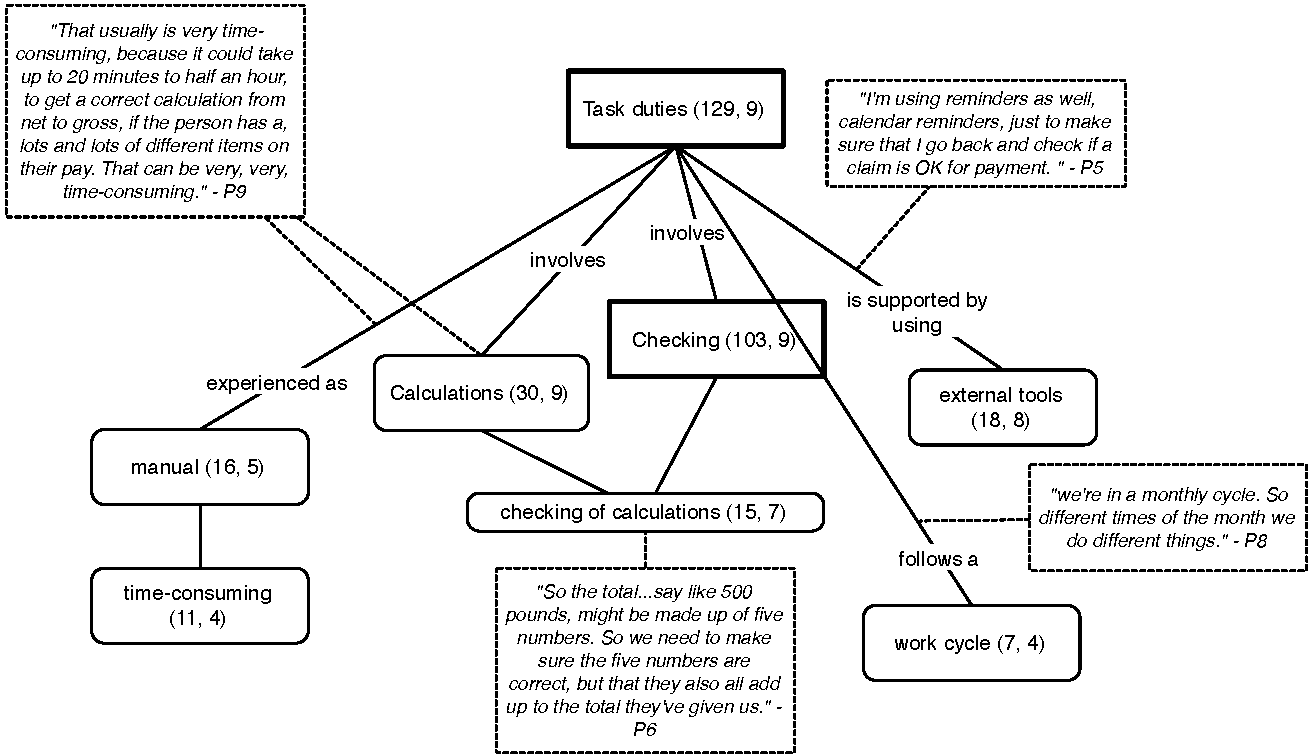
\includegraphics[width=\textwidth]{images/ch12/Task.pdf}
\caption[Study 1 Task diagram]{Diagram showing the theme Task. The numbers in parentheses indicate the number of quotes and the number of participants who mentioned it, respectively.}
\vspace{-9pt}
\label{fig:ch3_task}
\end{figure}
A common data entry task was entering expenses. Interviewees received expense claims from students and staff and had to check the information was correct. They then had to enter this data, along with other information such as budgetting and staff information, into a computer system.
All interviewees mentioned a large part of their job was checking that data was correct. In addition to transcribing and checking individual numbers, participants also mentioned they often have to perform and check calculations.
 Some tasks, such as calculations, had to be done manually and this was described as time-consuming. People used several external tools in their environment to support them in their tasks. For instance, P7 and P8 had paper sheets on their desk with information they frequently had to look up, so they could easily use this to check if the input they had received was correct.

Some people worked according to a work cycle, which meant they did different things at different times of the month. One week could be reserved for checking all the data they received from another department, while another week could be spent on solely inputting data. 

The time spent on each task differed: checking data on a short expenses form could be completed in two minutes, while a single calculation could take between 20 and 30 minutes. Two participants experienced dealing with a lot of data entry as tiresome.

\newpage

\subsubsection{Checking}\label{subsec:Checking}
\begin{figure}[!ht]
\centering
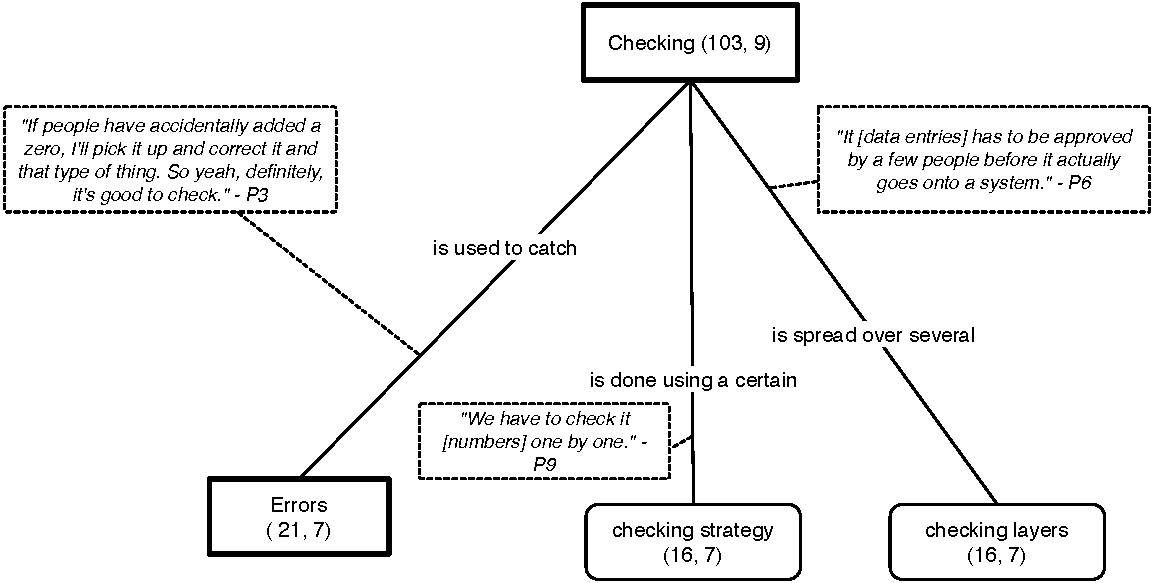
\includegraphics[width=\textwidth]{images/ch12/Checking.pdf}
\caption[Study 1 Checking diagram]{Diagram showing the theme Checking.}
\vspace{-9pt}
\label{fig:ch3_checking}
\end{figure}

All participants talked about checking data input for errors as a part of their job. Data was checked by several different people and departments before it was submitted. People's experience with this checking system differed: P3 felt that an error would be caught eventually because it goes through so many different layers, whereas P9 said it made people less careful about making errors and therefore they often received erroneous data. Sending wrong input back slowed the process down, and P8, who acted as the last person in his department to check before it gets submitted, warned that even with extra human checks not all errors get caught. 

People had to both check their own data input, as well as double-check other people's input. They maintained different checking strategies, ranging from checking each data item one by one to entering a group of data items first and then checking. 


\begin{table}[htp]
\centering
    \begin{tabular}{ | l | p{10cm} |}
    \hline
     \textbf{Participant} & \textbf{Quote} \\ \hline
    P3 & \textit{"we try and pick it [errors] up and then obviously there's all the different stages that pick it up as you go along."}\\ \hline
    P9 & \textit{"the departments actually sometimes treat us as a checking system [laughs], but they shouldn't really, the schools. Because we're here just to make sure that people get paid correctly. But even though we are like a second check, we feel sometimes that we are the first checkpoint."} \\ \hline
    P7 & \textit{"All this piece of work, when we input in the system, will be actually checked by another person... my manager will print it out, and then check... other colleagues will double-check it for you as well, the calculations."} \\ \hline
    P8 & \textit{"one of these errors could be things that are missed during the checking."} \\ \hline

    \hline
    \end{tabular}
    \caption[Study 1 checking quotes]{Verbatim quotes taken from the interview transcripts that were about checking.}
    \label{table:ch3_checkingquotes}
\end{table}%

\begin{table}[htp]
\centering
    \begin{tabular}{ | l | p{10cm} |}
    \hline
     \textbf{Participant} & \textbf{Quote/note} \\ \hline
    P1 &  first puts in all the details, then when done checks everything against the source. \\ \hline
    P7 & when entering numbers from paper to computer, mostly looked at paper form and the number pad; only looked at screen after finishing entering all the numbers from the form to check. \\ \hline
    P5 & \textit{"We would go by the receipt, so we would try to make sure that the receipts are in order."} \\ \hline

    \hline
    \end{tabular}
    \caption[Study 1 checking own input]{Checking own input when entering data.}
    \label{table:ch3_owninputquotes}
\end{table}%

\begin{table}[htp]
\centering
    \begin{tabular}{ | l | p{10cm} |}
    \hline
     \textbf{Participant} & \textbf{Quote} \\ \hline
    P5 &  \textit{"The numbers on the expense form will be checked individually. So the total will obviously be, say like 500 pounds, might be made up of five numbers. So we need to make sure the five numbers are correct, but that they also all add up to the total they've given us."} \\ \hline
    P6 & \textit{"The numbers on the expense form will be checked individually."}\\ \hline
    P9 & \textit{"We have to check it one by one."} \\ \hline

    \hline
    \end{tabular}
    \caption[Study 1 checking other people's input]{Checking other people's input.}
    \label{table:ch3_otherinputquotes}
\end{table}%

\clearpage
\subsubsection{System}
\begin{figure}[!ht]
\centering
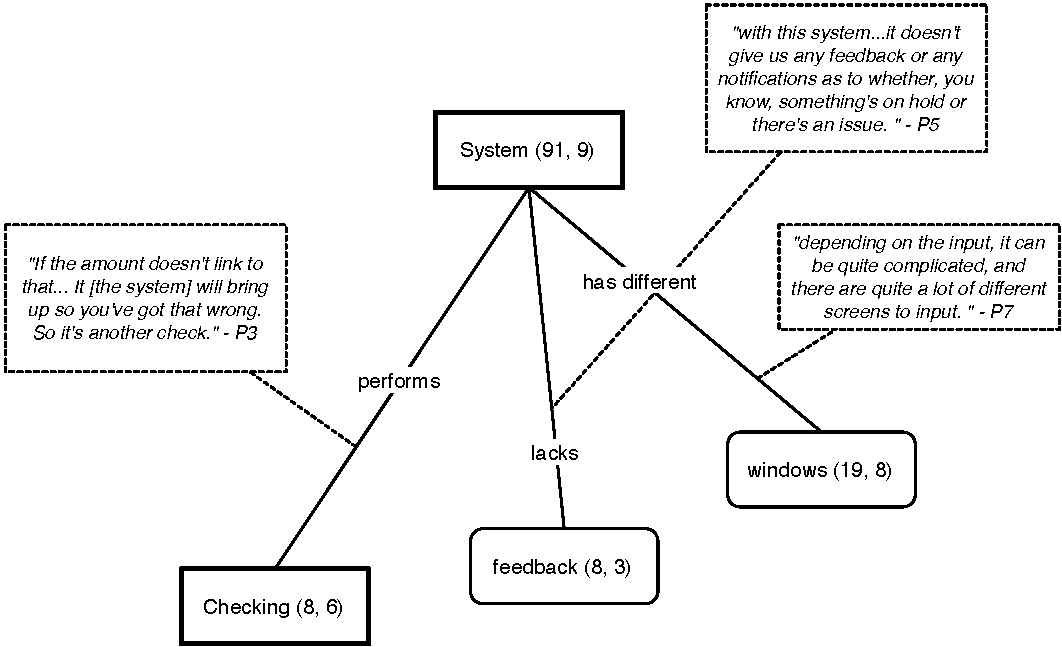
\includegraphics[width=\textwidth]{images/ch12/System.pdf}
\caption[Study 1 System diagram]{Diagram showing the theme System.}
\vspace{-9pt}
\label{fig:ch3_system}
\end{figure}

Data had to be entered into an information system on a computer. Some participants mentioned the system was another way to check for erroneous data entries: if the allowed number range of a variable was known, the system would let the user know if an out-of-range number was entered. However, it was also mentioned that one issue with the financial data entry system was that it did not give feedback if there was an issue or error.

The information needed for one task was usually spread over several windows on the computer, so sometimes people had to flick back and forth or memorise certain information from one window to use in another window. 

\clearpage
\subsubsection{Environment}
\begin{figure}[!ht]
\centering
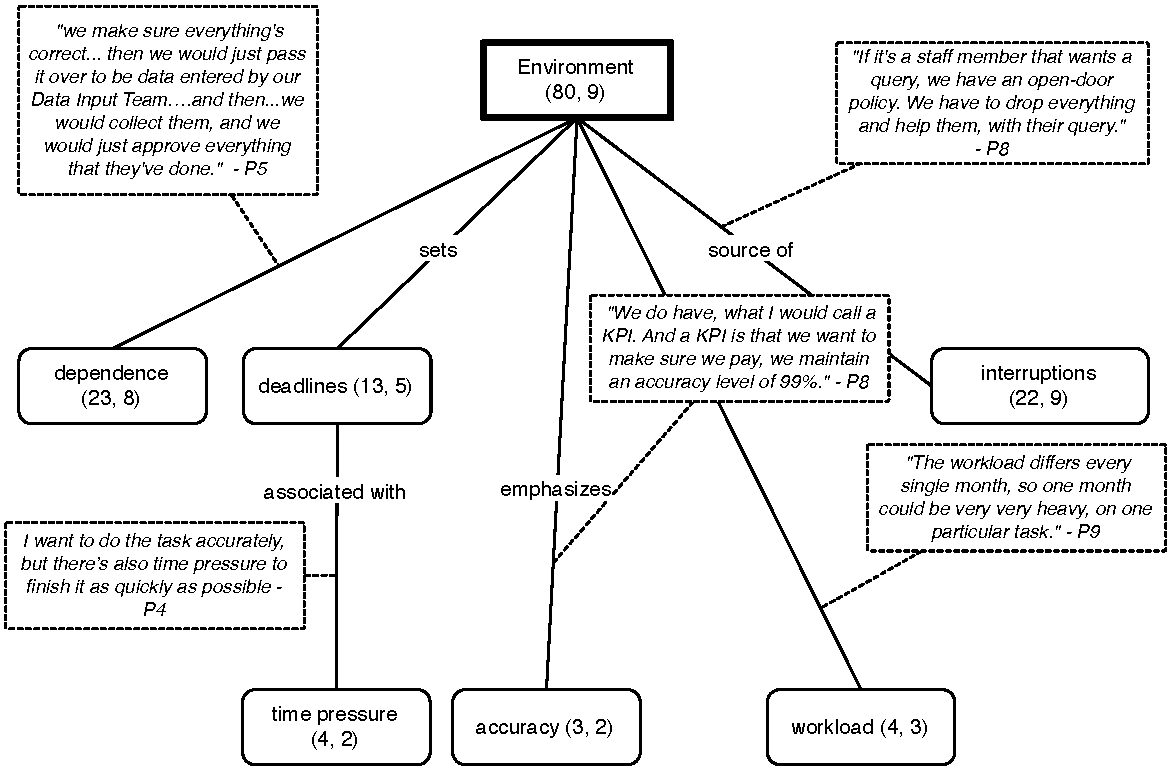
\includegraphics[width=\textwidth]{images/ch12/Environment.pdf}
\caption[Study 1 Environment diagram]{Diagram showing the theme Environment.}
\vspace{-9pt}
\label{fig:ch3_environment}
\end{figure}

Every time people described the environment they were working in, this was grouped under the Environment theme. The environment could be their immediate physical setting, or their organisation in general. 

All participants experienced interruptions during work. P8 mentioned he had to pause his task immediately if a staff member needed his help, but considered these interruptions part of his job. Other interviewees mentioned they tried to concentrate on the task at hand first, but did briefly attend to interruptions such as e-mail notifications, in case it was important.

People were dependent on other departments to finish a task. For instance, P5 checked paper expense forms, but did not enter these into the system herself. 

Some participants felt the pressure to be both accurate in data entry, as well as finish it quickly because of deadlines. The workload varied throughout the year.

\newpage
\subsubsection{Data}
\begin{figure}[!ht]
\centering
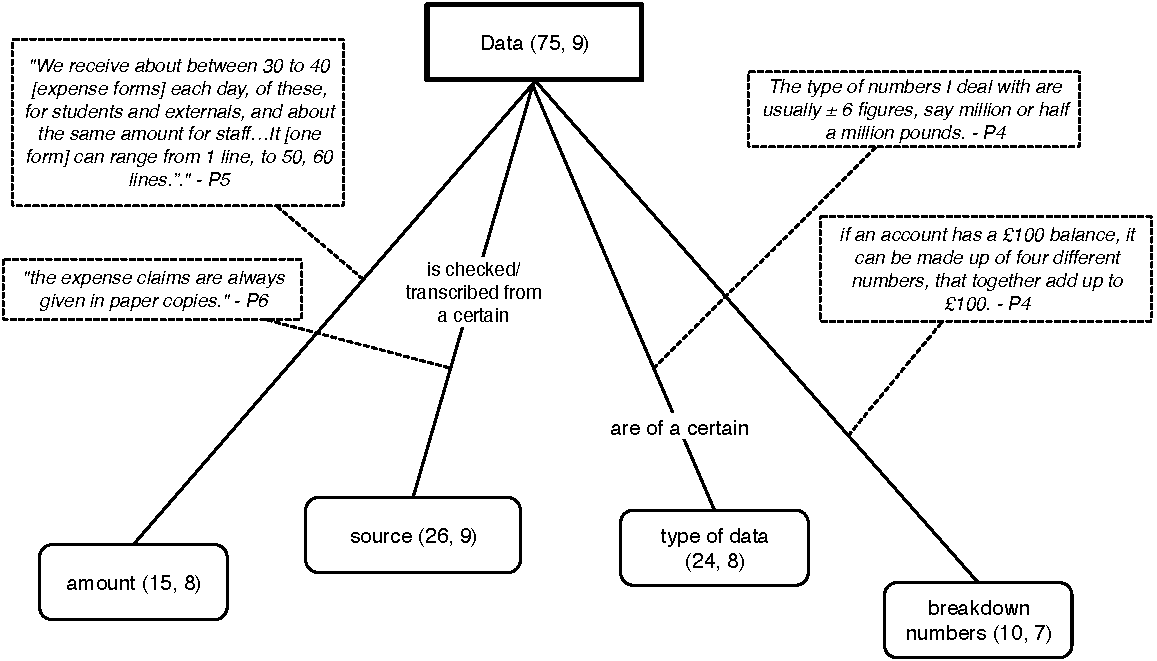
\includegraphics[width=\textwidth]{images/ch12/Data.pdf}
\caption[Study 1 Data diagram]{Diagram showing the theme Data.}
\vspace{-9pt}
\label{fig:ch3_data}
\end{figure}

Participants had to retrieve data from various sources. Some of the sources were electronic, such as Excel spreadsheets and Word documents. Some information had to be looked up in databases and work e-mails. Other information was received on paper sheets, and some participants had printed out information they frequently needed and had placed this on their desk. People had to transcribe numbers from paper onto a computer system for at least a part of their tasks. Some people worked with two screens.
The amount of data that people dealt with differed. P5 said that for expenses alone, the amount of numbers she received each day to check and input ranges from 100 to 6000 numbers.
People primarily dealt with numeric data, such as financial data and IDs. The monetary numbers they dealt with ranged from five to millions of pounds. Participants also entered and checked alphanumeric and non-numeric data such as employee names, addresses and bank account details.

Numeric data consisted of individual numbers, as well as groups of numbers that together made up a new number, such as the total amount of money spent on a project. Participants had to both check and transcribe each individual number, and check that the calculation was correct. 

\ \clearpage

\subsubsection{Errors}
\begin{figure}[!ht]
\centering
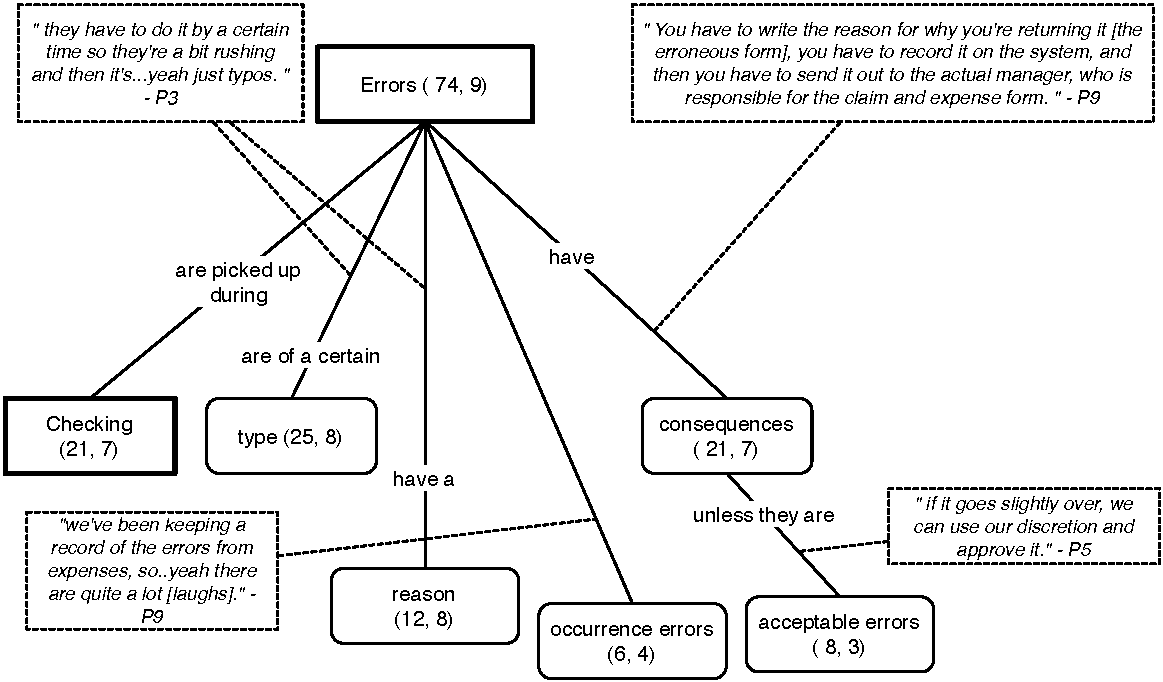
\includegraphics[width=\textwidth]{images/ch12/Errors.pdf}
\caption[Study 1 Errors diagram]{Diagram showing the theme Errors.}
\vspace{-9pt}
\label{fig:ch3_errors}
\end{figure}

Participants discussed that errors happened frequently, and talked about errors they spotted from other people. Visual checking was mentioned as the main method to catch and correct errors in time, but when possible the computer system sometimes checked for erroneous data as well. Errors that were made were typos, miscalculations, or people had the wrong information to enter. For instance, P7 mentioned that when salary rates change, employees often keep entering their old salary rate on claim forms, which then has to be corrected. The main explanation people gave for errors was that it is human to make mistakes, but it was also mentioned people are under time pressure, and that people rely on the fact it will be checked by another person, which makes them less careful in entering accurate data. 
If an error was spotted, this had certain consequences depending on if the error was acceptable or not. If the error was sufficiently small, it could be either processed or corrected without negotiation, but if it was a large error, it had to be sent back or forwarded to a higher authority for approval. 

P1 highlighted project IDs used to be letters but are now numbers, which are harder to memorise, and he felt it was easier to make a mistake. P4 worked with both paper and digital files to transcribe data from, but preferred digital files because he felt it was much easier to make an error and omit figures when transcribing from paper.

\begin{table}[htp]
\centering
    \begin{tabular}{ | l | p{10cm} |}
    \hline
     \textbf{Participant} & \textbf{Quote/note} \\ \hline
    P6 &  \textit{"it's quite common that we have to return an expense or payment back to someone. It happens quite often, yeah."} \\ \hline
    P4 & Yes all the time, lots of typos.\\ 
    \hline
    \end{tabular}
    \caption[Study 1 errors quotes]{People mentioned errors occur quite frequently.}
    \label{table:ch3_occurrenceerrorsquotes}
\end{table}%


\begin{table}[htp]
\centering
    \begin{tabular}{ | l | p{10cm} |}
    \hline
     \textbf{Participant} & \textbf{Quote} \\ \hline
    P3 &  \textit{"sometimes it's because people have done typos, done too many zeroes, or left out a zero."} \\ \hline
    P5 & \textit{"the expense breakdown doesn't match what (...) whatever they put as the grand total."}\\ 
    \hline
    \end{tabular}
    \caption[Study 1 type of errors quotes]{The type of errors.}
    \label{table:ch3_typeoferrorsquotes}
\end{table}%


\begin{table}[htp]
\centering
    \begin{tabular}{ | l | p{10cm} |}
    \hline
     \textbf{Participant} & \textbf{Quote} \\ \hline
    P9 &  \textit{"Because the departments actually sometimes treat us as a checking system [laughs], but they shouldn't really."} \\ \hline
    P7 & \textit{"Yeah, human laziness or something [laughs]."}\\ \hline
    P8 & \textit{"sometimes, you know, through human error, you know, things don't get paid properly."} \\
    \hline
    \end{tabular}
    \caption[Study 1 reasons for errors quotes]{The reasons for errors.}
    \label{table:ch3_errorreasonsquotes}
\end{table}%


\begin{table}[htp]
\centering
    \begin{tabular}{ | l | p{10cm} |}
    \hline
     \textbf{Participant} & \textbf{Quote/note} \\ \hline
    P5 &  \textit{"generally we tend, we try not to send claims back to departments because they might get lost in the post, and it's an inconvenience as well. So we try to... resolve it ourselves.."} \\ \hline
    P4 & We allow a certain amount of tolerance; if it turns out the thing you bought has actually decreased value and is now  \pounds40, we will allow to return  \pounds50\\ \hline
    P7 & \textit{"we normally e-mail the budget holder to say... what you authorised is actually different. But for this kind of thing, it's only 10 pounds...we normally just process this without contacting them."} \\ \hline

    \hline
    \end{tabular}
    \caption[Study 1 acceptable errors quotes]{Acceptable errors.}
    \label{table:ch3_acceptableerrorsquotes}
\end{table}%

\clearpage
\subsubsection{Strategy}
\begin{figure}[!ht]
\centering
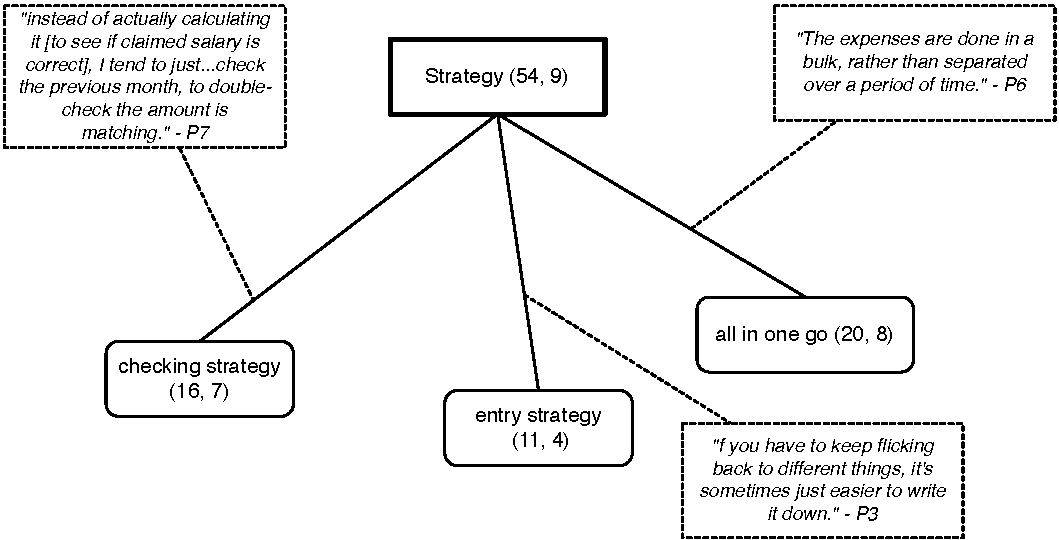
\includegraphics[width=\textwidth]{images/ch12/Strategy.pdf}
\caption[Study 1 Strategy diagram]{Diagram showing the theme Strategy.}
\vspace{-9pt}
\label{fig:ch3_strategy}
\end{figure}

Eight of nine interviewees saved up data to enter it all in one sequence. If they received forms with data input to check or enter, they saved these for later and then processed all the forms. P1 indicated he processed forms in batches of at least five forms, and found it disruptive to do just one or two and then switch to something else. 

P2 was the only interviewee that processed forms with numbers to enter as they came in, but did admit that if she had more data to fill in, she would probably do it in a more efficient way.

Some people said they preferred batching their work so that they entered all data into a single system at once because it is quicker and easier to do the same type of tasks in one sequence, and when that is finished concentrate on another task. P4 mentioned he does them all at once because he gets the forms in a bulk and feels pressure by his boss to finish them all immediately, rather than spread them over time. P6 explained he postpones processing expense forms until the deadline to submit forms for that month has passed, after which he does all forms in one sequence. 

People also talked about other strategies they used to do their job more efficiently. For instance, if they had to get out of the system to look up information digitally and then get back to the system window to enter it, they preferred to memorise the information, rather than flick back and forth and look it up each time they needed it. With numbers they had to enter frequently such as project codes, they memorised it even if they did not deliberately choose to do so. If the information to remember was complicated, they would write it down.

As discussed at the \nameref{subsec:Checking} section, people had different checking strategies and the number of times they looked back to the data source to check it against the data input varied. P7 said she sometimes deals with similar calculations, so she prefers to check the calculation she did last time rather than calculate it again. 

People explained that a lot of numbers they enter are calculated from other numbers. Some people liked to write out and keep a record of their calculation, in case someone had any questions on how that number was calculated.

\begin{table}[htp]
\centering
    \begin{tabular}{ | l | p{10cm} |}
    \hline
     \textbf{Participant} & \textbf{Quote/note} \\ \hline
    P3 &  \textit{"I just try and do it in the quickest way...It's nice, once you've done it, it's completed, so it's sort your weight lifted [laughs]. So you don't need to think about it again."} \\ \hline
    P6 & \textit{"the expenses are done in a bulk, rather than separated over a period of time. When I'm doing it lots at a time, I think once you get into sort of the hang of it, it gets done a lot quicker than..you just get used to putting them in, and inputting it all."} \\ \hline
    P9 & \textit{"I try to concentrate on my task...I try to do one task [i.e. doing all expenses], finish one, and then do another."} \\ \hline
    P4 &  It's difficult to take rests or even switch in-between number entry tasks because of the work pressure, and feels pressure by boss. \\ 
    \hline
    \end{tabular}
    \caption[Study 1 batching quotes]{Most participants entered all numbers in one go.}
    \label{table:ch3_inonegoquotes}
\end{table}%

\begin{table}[htp]
\centering
    \begin{tabular}{ | l | p{10cm} |}
    \hline
     \textbf{Participant} & \textbf{Quote/note} \\ \hline
    P3 &  \textit{" I wouldn't necessarily have to [memorise numbers], It's more just if you have to keep flicking back to different things, it's sometimes just easier to write it down, or just try and remember it. But you can obviously take the long version and keep flicking back to the correct screen."} \\ \hline
    P2 & \textit{"we have different grants and different project codes as a result, but you, because you use them so much, you end up remembering them."} \\ \hline
    \end{tabular}
    \caption[Study 1 strategy quotes]{Examples of strategies people used.}
    \label{table:ch3_strategiesquotes}
\end{table}%

\ \clearpage

\subsubsection{Importance of accuracy and paper trails}
\begin{figure}[!ht]
\centering
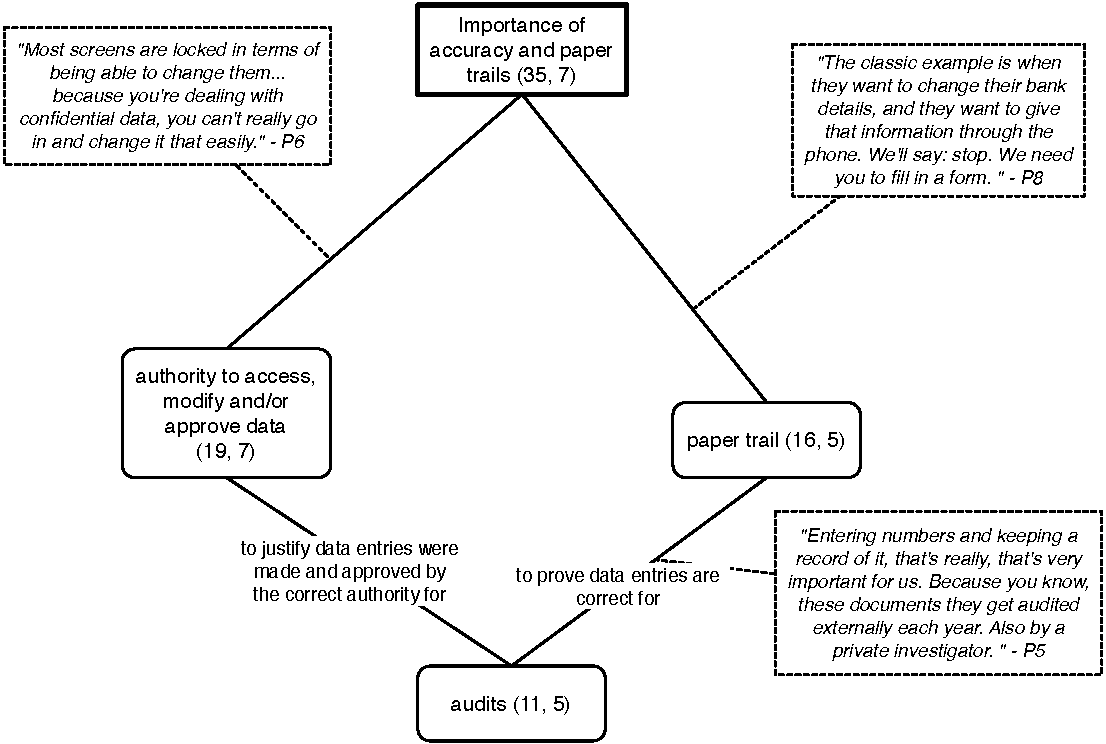
\includegraphics[width=\textwidth]{images/ch12/Papertrail.pdf}
\caption[Study 1 Importance of accuracy and paper trails diagram]{Diagram showing the theme 'Importance of accuracy and paper trails'.}
\vspace{-9pt}
\label{fig:ch3_papertrail}
\end{figure}

Because interviewees were working with sensitive financial data, another theme was importance of accuracy and paper trails.
Some data could only be entered in the system and modified by certain people.
Large figures had to be approved by a superior first before it could be processed, so it was clear to an auditor that expenses were made with the correct approval.
Hard copies of data had to be archived and were checked by external auditors. For instance, all expenses were claimed on paper forms, and had to have the original receipts as evidence that the expense claims were correct. Some data could not be given over the phone but had to be written down and sent via a paper form.

\pagebreak

\subsubsection{Other}
\begin{figure}[!ht]
\centering
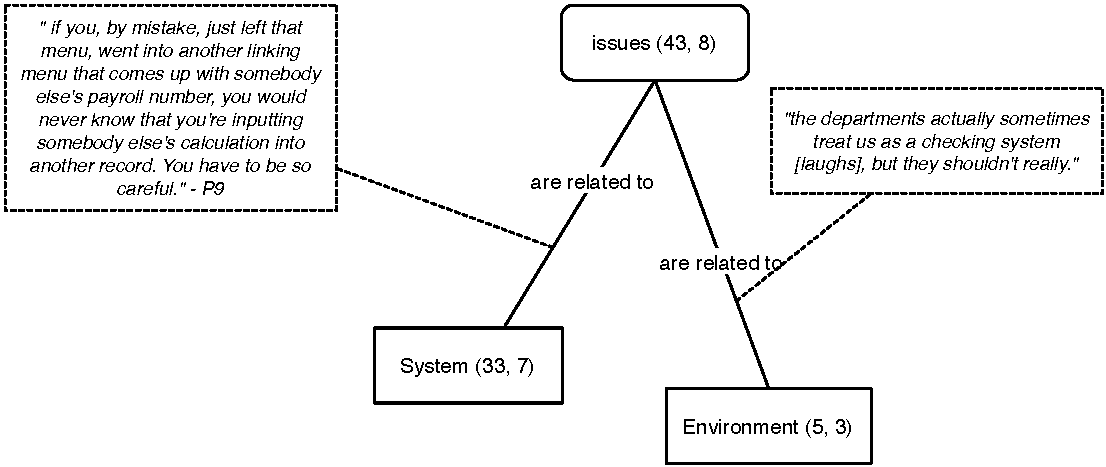
\includegraphics[width=\textwidth]{images/ch12/Other.pdf}
\caption[Study 1 Other diagram]{If people described issues, it usually had to do with the system.}
\vspace{-9pt}
\label{fig:ch3_other}
\end{figure}

Interviewees mentioned several issues they experienced. Most of the time, the issues had to do with the current data entry system they were using. P7 mentioned number entries on the computer screen were small and hard to read, and could not be enlarged. P5 mentioned she did not get notifications from the system if there was an issue with a payment, so she would not know about it until staff members would call up to complain they had not been paid yet.  Other issues had to do with the organisation, such as the experience that the multiple checking layers made people rely on other people to check their input.

\begin{table}[htp]
\centering
    \begin{tabular}{ | l | p{10cm} |}
    \hline
     \textbf{Participant} & \textbf{Quote/note} \\ \hline
    P5 &  \textit{"There are other issues. You could say I think hundreds, I mean not just with the work that we do on expenses, but across [university A], across [university A] Finance, the Finance division...We just have to kind of work our way around the system and you know, adapt to it."} \\ \hline
    P7 & \textit{"It's only the matter of how you get used to the Payroll system. Because companies have different systems, the data inputting can take a while to get used to it."} \\ \hline
    P9 &  \textit{"You know, all systems are a bit funny, I think. But you just gotta get used to it."} \\ \hline
    \end{tabular}
    \caption[Study 1 issues quotes]{Issues that participants experienced with the system.}
    \label{table:ch3_otherquotes}
\end{table}%

\pagebreak

\subsection{Discussion}
The purpose of this study was to gain a better understanding of the type of data entry tasks in financial offices, and the physical environment in which these are conducted. For this purpose nine interviews were conducted with staff from two public universities who worked with financial data. The main findings of the study are: 

\begin{itemize}
\item 
people have to get the data to enter from various sources, with varying information access costs
\item 
people batch their work to enter a lot of data entry at once, and minimise switching between tasks. 
\item 
data entry errors are common, and the current solution is to have data entered and checked by multiple people before it gets submitted to the system
\end{itemize}

\subsubsection{Information sources and access costs}
A prevalent data entry task of participants' work was processing expense claims from university staff and students. A substantial part of this task is not just entering the data but also collecting it from multiple sources. For example, the expenses had to be entered from paper forms and receipts, foreign currencies had to be converted and copied from a website, and staff and financial information had to be retrieved from sources such as electronic spreadsheets, databases and e-mails. 
In data entry experiments, the data is often shown on a computer, to make it easy to manipulate. This was sometimes the case in the office setting studied here, but data was also transcribed from paper sheets into a computer. Furthermore, in lab experiments people are often only presented with the data they have to enter and sometimes are given only one data item at a time. The sources from which people had to enter data in this study usually contained a lot of data, not all of which was relevant to the task. The amount of irrelevant data on the sources can increase the time people need to look up the information they need.

The cost to access the information sources differed. For instance, some paper sheets were on people's desk, but some paper sheets had to be retrieved elsewhere. Sometimes participants had to go through a large spreadsheet, before they found the number they needed to copy. Participants also dealt with multiple windows on their computer screen, and sometimes needed to switch between different windows. Instead of flicking back and forth to view information they had to enter in another window, people said they preferred to memorise it. This supports previous research which showed that people make strategic use of internal and external resources and do not always maximise off-loading cognition to external resources \citep{Gray2006}. Even though participants were aware they did not have to remember information, they found this easier and faster rather than looking it up or writing it down. 

This strategy allows people to be faster, but carries the risk that they misremember it. In previous studies, trying to hold more items in memory during a copying task increased errors \citep[e.g.][]{Morgan2009}. However, in these studies people had to copy over coloured blocks, which were abstract to the participants and may have been too hard for participants to memorise \citep{Waldron2011}. In the current study, the information had some meaning to the users, and even if they were dealing with abstract information, such as project codes or ID numbers, some items were entered more often than others. Participants mentioned that even if they did not make a conscious effort to memorise these, they had to enter these numbers so often that they ended up remembering them. This is in line with prior findings that some numbers are more familiar than others, and that these familiar numbers are more strongly represented in memory \citep{Wiseman2014}. 

If information to copy is familiar and contains numbers and text, making the effort to encode the information more deeply has been shown to make people more accurate \citep{Gray2004, Soboczenski2013}. It is therefore not clear if the effect of a memory-based strategy on accuracy, as found in \citep{Morgan2009}, would extend to copying the material of this study.

People used some external tools to aid memory. For example, some participants had printed sheets with information they used and entered often, so they did not have to repeatedly look this up in the system. They also used calculators and pen and paper to perform calculations.

\subsubsection{Batching data entry tasks}
Eight of nine participants batched data entry tasks to do them all at once, rather than spread them over time. The only participant who processed expense forms as they came in said she did not receive a large amount of forms. She explained that if she dealt with a higher volume of expenses, she would probably do it in a more efficient way.

There were different reasons behind the strategy to enter a large amount of data in one sequence. One participant received forms in a bulk, and felt time pressure to finish them all at once, rather than spread them over time. The other seven participants said they received forms on an ad-hoc basis, but deliberately saved them until a specific moment and then processed them all in a bulk. They preferred to focus on one task at once, and some people stated that it made them faster in entering data after a while. 

This is consistent with Healy et al.'s \citeyearpar{Healy2004} study, where learning effects could be measured in a number entry task. However, in their experiment participants became faster but also more erroneous in entering data. In the current study, P3 mentioned that most of the errors she picks up from colleagues are typos caused by rushing to finish the task. P4 mentioned that he wants to enter numbers accurately, but that there is a time pressure to finish things in time. This is in line with the speed-accuracy trade-off discussed in literature, and that a sense of urgency may cause people to enter numbers faster but at the expense of a higher error rate \citep{Lin2011, Lin2013}.
\citet{Healy2004} recommended regular breaks when entering large amounts of data to maintain accuracy, but P4 in the current study explained it is difficult to initiate breaks himself, when he feels a time pressure to finish it.

\subsubsection{Multiple checking stages}
In order to prevent errors, input was entered and checked by multiple people before it was allowed to be submitted into the system. This checking method is similar to \citeauthor{Reason1990}'s \citeyearpar{Reason1990}  Swiss Cheese model, where multiple checking layers are used to minimise the risk of errors. However, as a result of this people seemed less careful in checking their own input, because they knew it would be checked by someone else. 

In previous studies, providing incentives for people and introducing lockouts into the data entry interface has been shown to influence how carefully people check their input \citep{Li2015, Gould2015}. The findings from the current study suggest that how and whether people check also partly depends on what the primary objective of their task is: entering or checking input.

When people were asked to check other people's data input, they checked each data item one by one. However, when they had to enter data themselves, they tended to chunk data items and only checked their entries when they had entered all items on one source. This finding is based on both observations when participants demonstrated a number entry task, as well as descriptions people gave on how they tend to perform their task. When people are asked to enter data, checking their input is not the main focus of the task, but rather a post-completion step that has to be performed after the main goal of entering data has been completed. It is well known post-completion steps are prone to errors, as it is not part of the main goal of the task \citep[e.g.][]{Byrne1995, Li2006, Li2008}.

It could also be that people were aware their input was going to be checked by another person, and therefore did not spend as much effort trying to check it properly. When talking about checking other people's input, people emphasised how it was important that each data item was checked carefully. However, when they talked about their own input, they tended to emphasise this less and mentioned another person would double-check it anyway.

\subsubsection{Summary}
The purpose of this study was to get a better understanding of data entry tasks associated with finance administration office work, and the context in which these tasks are done. While it was informed by previous data entry research, it did not have a particular theoretical framework prior to undertaking the study to inform and guide the data collection and analysis. 

A prevalent data entry task of the participants was processing expense claims from university staff and students. A substantial part of this task was not just entering the data, but also collecting it from multiple sources with varying information access costs. As my data collection and analysis progressed, it emerged that framing the findings in terms of different information access costs (IAC) of these information sources had the potential to provide a useful lens on the data for informing the design and evaluation of data entry systems. As the study looked at the wider context of participants' data entry work and did not focus on entering expenses per se, it was not recorded which sources people needed and how they looked up information.

The aim of the next study is to investigate the information sources people need for an expenses task, and how they currently manage subtasks of looking up information from an expenses task. 
%Sometimes the cost to access an information source was low, and people could easily access it and look at it while entering it. Other times the cost was high, and people had to go back and forth between the window that showed the information, and the window in which they had to enter the information. Theory suggests that these different access costs have an impact on strategy, speed and accuracy. In previous experimental studies, an increase in IAC made people check the information source less and instead enter what was in their head. This can make people more efficient as it minimises switching between the information source and the input interface, but if the information in the head is wrong, it increases errors. In these previous studies, it increased errors, but the studies made use of abstract artificial information, which may have been too hard for participants to memorise. 
%In the current study, people had to copy numbers and text. Previous studies showed that when looking at text and/or numbers, a deeper encoding of the information in memory makes people more accurate in entering the information. 
%The next study aims to see if the effect of IAC on a copying task extends to copying numbers, which people have experience with copying and can more easily memorise.

\section{Study 2: Information sources for entering expenses}

\subsection{Introduction}
A large part of data entry work studied in Study 1 was not only entering the data, but retrieving it from the environment. People had to leave the data entry system to look up information from several sources, and hold data in memory whilst switching between documents, applications and the data entry system. 
The purpose of this study is to investigate people's current work practices to look up information from the environment for data entry work. What information do they need, and what information sources do they use? And how do they address these needs? Do they look up information as they need it, or get all the required information first and then enter it? It is important to understand how people manage subtasks of looking up information as part of data entry work, as different strategies impact task performance. 
%They may also change their strategies as they get more experienced with the task and know where to get the information from, or enter all information that is easy to access first.

The following questions will be addressed in this study:

\begin{enumerate}
\item 
What is the information needed for an expenses task?
\item 
Where is this information retrieved from?
\item 
What are the strategies people use to look up information?
\end{enumerate}

A contextual inquiry was conducted with nine finance employees from the same population as in Study 1. In this study, the specific focus was on people's information behaviour. Participants were observed at their workplace, and asked to first carry out a data entry task while thinking out loud. Next, they were observed while they continued working as they would normally.

Participants in the current study were video recorded while doing the expenses task. The video recordings captured the participants' interactions with the artefacts involved in the task, but the financial data on the information sources could not be identified from these recordings. The video recordings were used to supplement written observation notes, and after the observation part of the study, some video segments were played back to participants to explain what they were doing at certain moments.

Data was gathered and analysed using Distribution Cognition (DC) as a theoretical framework \citep{Hutchins1995}. Distributed Cognition is a theoretical framework that views cognition as distributed between people, internal and external sources and over time. 
As it takes the distributed nature of cognition as focus of analysis, it was considered it to be a useful framework for this study to help make sense of the fragmentation of, and access to, information for data entry work. 

%Despite the usefulness of DC in understanding and designing for human-computer interactions \citep{Hollan2000}, to my knowledge it has not yet been applied to data entry work. %In most data entry studies, information is given and well-defined. The focus then becomes on decreasing the access costs []. However …

To analyse the data, I followed the guidelines of \citet{Furniss2006} on constructing descriptive models of the task environment. Though the models were originally developed to apply Distributed Cognition for teamwork, the models can also be useful with an individual as the focus of analysis. In particular the Physical and Artefact model were useful in understanding the distribution of, and access to, information for the user. The methodology facilitated to identify potential issues, and better understand people’s current strategies and workarounds. 
%This study focused on understanding how information is laid out in the environment for data entry work at financial offices, and people'��s current practices to collect information, with the aim of informing design of user-friendlier systems.

\subsection{Method}
\subsubsection{Participants}
Nine participants (five male) from four different finance offices took part in the study. 

Participants from Study 1 were invited to participate again, but only one participant was able to participate again in the current study (P8 in Study 1, P1 in Study 2). 
For the remainder of recruitment, a parallel sampling approach was taken \citep{Onwuegbuzie2008}. This means participants were drawn from the same population using the same recruitment techniques, but were not the same individuals. As in Study 1, they were employees from financial offices at public universities dealing with processing expense claims. Participants had one of the following roles: research manager, payroll officer, and administrator.

People were recruited through a combination of convenience and snowball sampling. People were invited to participate via emails sent to opt-in mailing lists of Finance departments, and emails forwarded by contact persons and people who had already participated. A session with a single participant took between 2 and 2.5 hours, and participants were reimbursed with \pounds15.

\subsubsection{Site setting}
The study took place in the same type of office setting as in Study 1. Participants were recruited from the same two public universities, and one office from Study 1 was visited again in this study. The other participants were from three different offices within these universities. They worked in open plan offices with two or more colleagues working nearby. 

\subsubsection{Contextual inquiry}
My data collection was informed by using the methodological approach of contextual inquiry.
Contextual inquiry is a combination of observation and interviewing users and their everyday work, with the aim to use the findings to inform design of the systems they use \citep{Holtzblatt2014}.
\citet{Holtzblatt2014} argue that observing participants carrying out their work can reveal concrete details, and it can help participants to recall past situations of carrying out work. It is therefore considered to be an appropriate method for the aims of this thesis, as it involves understanding users' expenses work with the aim to translate it into design implications for their expenses system. 

All interviews were audio recorded, and observations were audio and video recorded. The contextual inquiry consisted of four parts \citet{Holtzblatt2014}:
\begin{enumerate}
\item 
Interview

In this part, the participant was asked general questions about their work. This part was primarily to make the participant feel comfortable and start the session easy. As I had already gained an insight on finance employees' general work in Study 1, this interview was shorter and more particularly focused on their expenses task and information sources they used. 
\item 
Transition

In this part, the participant demonstrated the expenses task while thinking out loud. I prompted the participant to elaborate what was happening if the participant fell quiet, or if something interesting or unusual happened.
\item 
Observation

During this part, the participant continued doing his/her work without being interrupted or explaining what he/she was doing and why. I observed and made notes.
\item 
Summary

In the final stage, I summarised to the participant what I had found to check if these assumptions were correct. If some parts of the observation need clarification, segments of the video recording were played back to the participant, and he/she was asked to explain what was happening at certain moments.
The participant was thanked and debriefed.
\end{enumerate}

\subsubsection{Pilot study}
In order to test the suitability of the study set-up, a pilot study was conducted with a financial administrator at a university who dealt with processing expenses. The study took place at the university, and notes were taken with pen and paper. 

Initially, the intended method of this study was to conduct a contextual inquiry, followed by a week-long diary study where office workers would log diary entries of their expenses tasks. The aim of this diary study would be to get a further insight in additional information sources they may sometimes use, that were not covered in the contextual inquiry.  Participants would submit a diary entry either by writing down a description or by taking a photograph of the task setting, showing the information sources. At the end of the day, they would have to answer the following questions about their short entries: what information did you need, where did you need to get it from, and when did you look up the information. This method built on a study by \citet{Sohn2008}, where participants kept a diary of their mobile information needs and how they addressed those needs. 

The administrator explained that expense tasks usually are conducted in the same manner, and predicted I was unlikely to find a lot of instances that differ from my observations of having office workers do the task.
Furthermore, by observing them I am able to see the access people have to the resources and how much time it takes them to get the data, as well as when in the task they decide to look up information. This information would be more difficult to get insight to through diary entries.

It was therefore decided after this study to not conduct a diary study but instead only observe office workers, and ask them to explain their work.

\subsubsection{Ethical considerations}
The study has ethical approval from the UCL Research Ethics Committee [Project ID Number UCLIC/1415/001/Staff Brumby/Borghouts]. 

Participants were invited by email. The email included details such as the purpose, duration and reimbursement, and what participation would involve. 

Before the start of each session, participants were again verbally briefed about the purpose of the study, and what would be expected of them. They were then asked to read and sign a consent form, and were given an information sheet with the study information and my contact details for them to keep. 

All participants gave permission for the session to be audio and video recorded. After the video camera was set up, participants were shown what was captured by the camera, to confirm the camera was set up appropriately. This ensured the participant that no financial data was legible from the recordings.

It was explained that the purpose of the study was to get a better understanding of how they normally go about their work with an aim to improve the system, and that there were no right or wrong ways of doing tasks. They were free to withdraw from the study at any time.
Participants were informed that the data would be used for research purposes only and stored in accordance with the Data Protection Act 1998. Names of participants and the organisations they were working at were not included in interview notes and transcripts.

Video recordings were not only used to supplement audio transcripts and written observation notes, but were also used in debriefing interviews.
If something interesting or unusual happened during the observation, a video clip of this moment was played back to the user in the debriefing, and they were asked to elaborate on this moment.

The use of video recordings to aid recall in the debriefing interviews was inspired by \citet{Cangiano2009}, who captured screen recordings to capture workers' activities in a law office. In debriefing interviews, they played these recordings back to the workers, and asked them to explain their activities. The recordings were useful for workers to accurately recall what they were doing at the captured moments, and why they had certain windows open. 

Screen recordings provide a more detailed account of activity than video recordings, however there are also privacy issues and not all participants agree their activity to be recorded \citep{Rule2015}. Due to confidentiality issues to share financial data, it was not possible to use screen recordings in this setting.

\subsubsection{Data collection and analysis}
All sessions were audio and video recorded. 

Every time the participant used an artefact, I asked them to show it to me. Artefacts included paper, a computer program, a tool such as a calculator, or a spreadsheet. I wrote down a quick description of the artefact and where possible, a photo or screenshot was taken of the artefact. 

Screenshots were made of the data entry system participants used to enter the expenses data These screenshots did not include any data entries.

In addition to video recording the think-aloud and observations parts, I made notes by hand. Whenever something interesting happened during the observation part, I made a note of it to remind me to ask the participant questions on this in the debriefing interview.

Data was analysed using a Distributed Cognition (DC) perspective. I used \citet{Furniss2006}'s guidelines in developing the following descriptive DC models:

\begin{itemize}
\item 
The physical model: this model describes the physical layout of the task environment
\item 
The information flow model: this model describes how information flows through all users involved in the task
\item 
The artefact model: this model describes all artefacts involved in the task
\end{itemize}

These models are based on the working models of contextual design to identify work activities, but are more focused on how information is distributed in the environment. Each model consists of a diagrammatic representation that visualises the data, and a narrative representation which verbally describes the data.

After each data collection session, written notes were typed out and any initial thoughts or findings were added. After data collection from the first four participants, initial versions of the models were made. Making these initial versions helped identify any gaps in the data collected so far, and helped guide further data collection sessions.

Audio recordings of the interviews and think-aloud verbal protocols were transcribed verbatim. Video recordings were played back, and additional notes were made if anything new was observed by watching these video recordings.

The written transcripts and notes were read and if a quote or note was relevant to one of the models, it was grouped under that model. The groupings were reviewed and used to refine and expand the models. Video recordings were consulted to fill any gaps from the written data.

%The models gave an insight in people's current task environment, and highlighted several issues. %which were grouped into three themes: lack of established coordination mechanisms, design of artefacts, and limitations in communication bandwidth.  In order to identify patterns of information strategies the models, transcripts and notes, were reviewed and all findings that related to people's strategies were grouped in a separate category. 

%
%\subsubsection{Expected findings}
%Based on findings from Study 1 and previous work on the influence of information access costs on task strategies \citep{Gray2006}, I expect the following findings:
%
%\begin{itemize}
%\item
%People will have to switch multiple times between different data sources as part of the same expenses task.
%\item
%The IAC of these data sources varies. 
%\item
%If IAC of an information source is high, people will rely more on knowledge in the head: they will copy over more data in one go when IAC is high.
%\item
%Batching is a task planning strategy that gets employed by people with some experience in the task, in order to reduce switching between data entry tasks, and other tasks.  People will save up data entry tasks to do them all in one sequence.
%
%Depending on people's experience and awareness of how costly it is to access information, people may plan their expenses task to reduce switching between entering and looking up information. They choose to enter all the low-IAC items first, in a batch, and then the high-IAC items second, also in a batch, rather than looking up each item as they need it.  An explanation for this is that they minimise the start-up costs of the entry task.

%\end{itemize}

\subsection{Findings}
I used the DC principles as described by \citep{Furniss2006} as guidelines to decide what to include in the models. The principles of each model are described at the start of each section, and marked in italics (e.g., \textit{horizon of observation}) in the narrative descriptions.

\subsubsection{Physical model}
\begin{figure}[!ht]
\centering
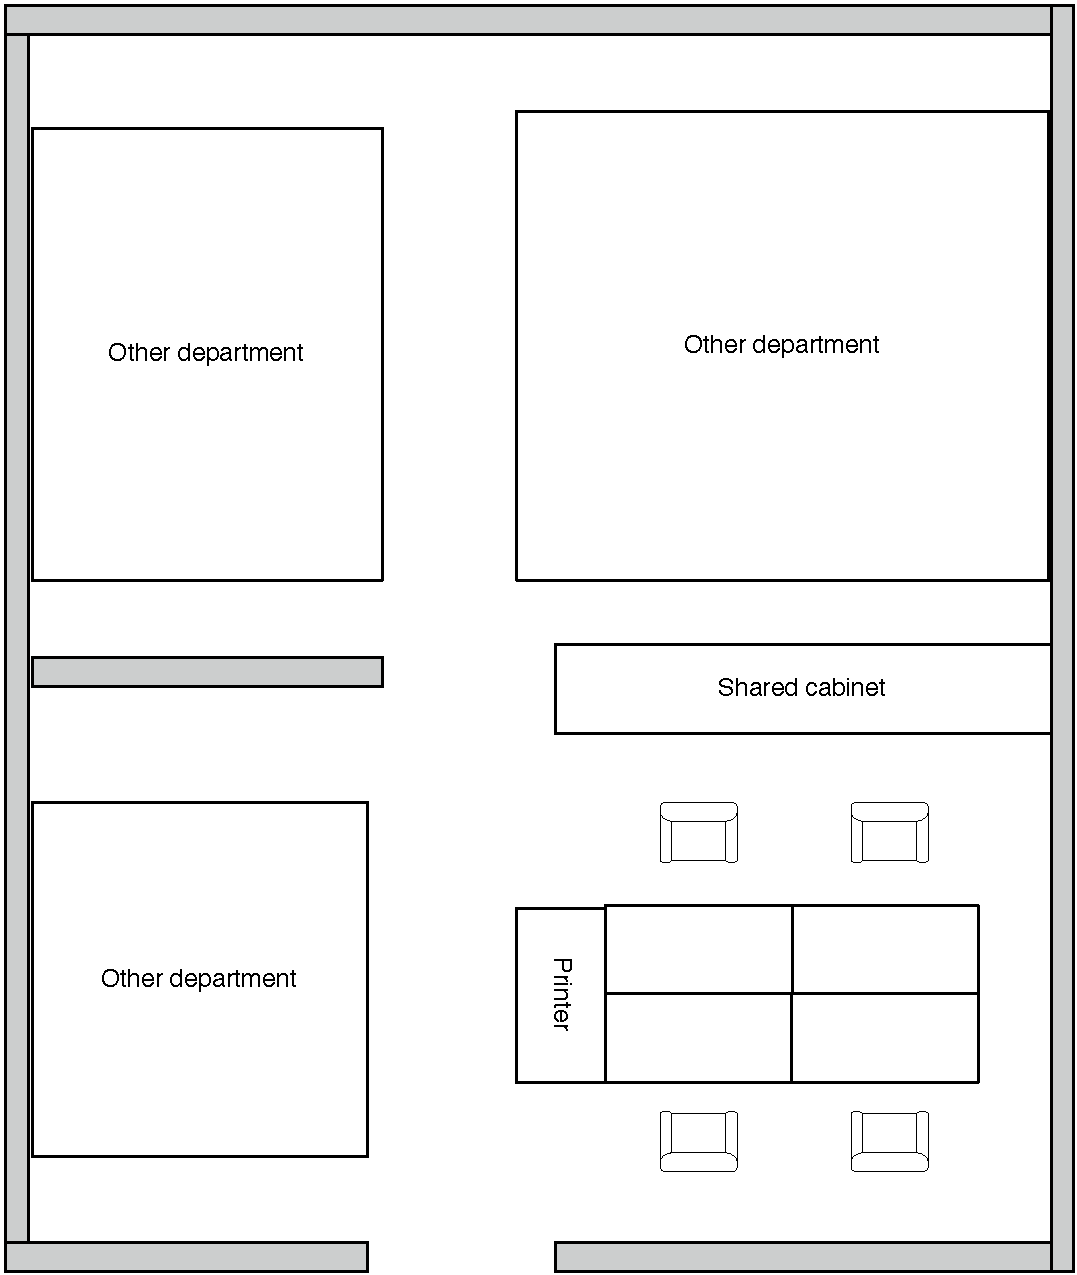
\includegraphics[width=0.3\textwidth]{images/ch12/ch12_physmodroom.pdf}
\caption[Study 2 Room model]{Physical model diagram showing a typical physical layout of people's work environment at room level.}
\vspace{-9pt}
\label{fig:ch12_physmodroom}
\end{figure}

\begin{figure}[!ht]
\centering
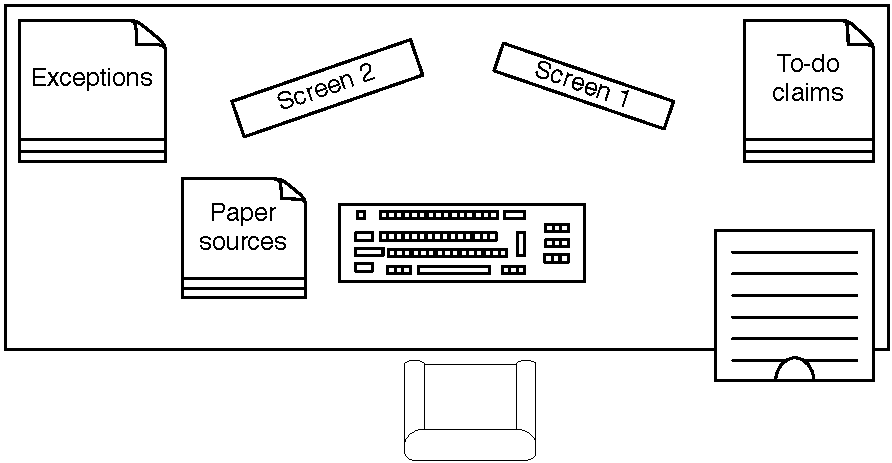
\includegraphics[width=0.3\textwidth]{images/ch12/ch12_physmoddesk.pdf}
\caption[Study 2 Desk model]{Physical model diagram showing the physical layout of people's work environment at desk level.}
\vspace{-9pt}
\label{fig:ch12_physmodroom}
\end{figure}

The physical model describes what the individual can physically hear, see, and access, and how information sources are laid out in the physical environment. In developing the model the following was considered: what is the proximity of, and access to, devices and people: what can be seen and heard from the individual's point of view?

\begin{framed}\noindent
\textbf{Physical model principles}

\begin{itemize}
\item Space and Cognition: how do people use the physical space to support their work
%\item Perceptual principle: what is the mapping between the spatial layout of information, and that which it represents
%\item Naturalness principle: does the form of how information is represented match the properties of what it represents
\item Subtle bodily supports: do people use their body to support their work
\item Situation awareness: are people informed of what is going on
\item Horizon of observation: what are people able to see and hear
\item Arrangement of equipment: how do people arrange their equipment
\end{itemize}

\end{framed}

%Physical layout
The physical layouts of the four offices were not identical, but shared a number of characteristics. All participants had their own desk and worked in an open office with two or more colleagues. P3 was the only person in the office responsible for data entry tasks. The other eight participants had colleagues in the same room who dealt with similar tasks. P1, P2, P8 and P9 also had colleagues in the same room that worked on different tasks. Colleagues that were working on different tasks were situated further away from them than other colleagues. As an example, the physical environment of the office of P1 and P2 is depicted in Figure \ref{fig:ch12_physmodroom} at room (a) and desk (b) level. The number of people in one room ranged from two to sixteen. 

The open layout made it easy for colleagues to interact with each other and share information between themselves. They could see when a colleague was present and available to consult. Participants regularly consulted colleagues in their room to retrieve information they could not find on any other sources. This information is given verbally, or a colleague directs the participant to the correct information source.

The offices had an open-door policy, meaning that workers could at any time be interrupted by people walking in. During the observations, participants were regularly interrupted by colleagues. They responded to it but used \textit{subtle bodily supports} to not lose track of where they were in the expenses task. For example, P3 responded verbally to a colleague but kept his kept his visual attention on the computer and tried to continue with the expenses task. When P1 was interrupted by a colleague, he placed a finger on the computer screen to remember where he was in the task.

%Sometimes it is colleagues at the same level of processing, sometimes it is people who are higher in the task hierarchy. For example, a boss who needs to check another colleague'��s entries can be collocated around a desk and query this colleague if something is incorrect. They can also view how many of the outstanding claims still need to be processed as they are on their colleague's desk.

%SOURCES
All participants worked with both paper and digital information sources. Several participants used the physical \textit{space} to organise their paper sources. P2 maintained separate physical locations on his desk for expense claims to be processed, expense claims that had been completed, and exceptional claims that required further attention. P7 also had paper sources fixed on his wall, which were visible from his desk. 

Other physical sources were located in an individual's drawer, in a shared bookcase or drawer in the same physical room. These were not visible from their desk, and participants had to physically move from their desk to retrieve and view this information. Participants could see whether a colleague is present or not, and whether they can consult them at that moment to request information. Recent physical files are kept in a closet in the same room, whereas older files and employee files are physically kept in another location. These older files were used less frequently.
If P6 received expense claims, she placed these in her drawer to return to later. If there were a lot of claims to be processed or if the participant started processing claims, these were placed on their desk. 

Participants become aware of new claim requests by batches of claim forms or receipts on their desk with a handwritten note, the claimant asking them in person, or when they check their e-mail and see a new e-mail by the claimant. For physical claims, they browse through them and place them either at a dedicated area on their desk or in their drawer, to return to later. P2, P3 and P6 re-ordered claims based on urgency. Claims that were more urgent were processed first. These could be claims by their boss, or claims with an explicit instruction that it was urgent. In addition, P2 sometimes grouped claims according to category. The reason for grouping them is that different categories of expenses can require other data fields to be filled in, and P2 felt it to be easier to do these particular type of claims together. Examples are travel expenses for which participants have to fill in the departure point and destination, or external lunches for which the name of the restaurant has to be filled in. Participants place exceptional claims in a separate physical location. For P2, this was in a separate tray in the top-left hand corner of his desk. By putting it in his \textit{horizon of observation}, he can see if there are still claims in this tray to be processed and return to at a later point in time. P2 starts each day by seeing if there are claims in this tray, and processes these first. P5 places exceptional claims in a separate drawer. They are not visible and she does not use any reminders, but returns to these when she sees fit.

Participants also received requests digitally through email. They could not place these in their horizon of observation. However, whether the claim requests were in physical or digital form, they always needed the physical receipts of expenses, before they could process a claim. Similar to physical claim forms, they had these receipts either in their drawer or on their desk, as a reminder that they still needed to process these claim requests.

Participants also created their own artefacts to aid them in their work. This includes physical artefacts, such as a spreadsheet with frequently used codes, as well as digital artefacts, such as a digital form to look up codes by person name. Participants could type in a name of a claimant, and the form populated codes related to one person. This made it easier for people to look up which account codes to charge the expenses to. 

Digital information sources included the data entry system, intranet, and external websites via their computer. Furthermore, they had digital files, such as PDF files, Excel spreadsheets, and Word documents stored on their desktop computer. The \textit{arrangement of equipment} was that seven out of nine participants had two screens. All seven participants mainly used one screen, both to enter and retrieve information. Some participants used a second screen to display their email inbox. If they received a notification of a new email, they would briefly glance to determine the urgency and importance of the email, but would try to continue with the expenses task. 

Sometimes a claim was checked by multiple people in the same room. Participants had \textit{situation awareness} of the progress of the claim as long as it was still in the same physical office. They could see the progress of expense claims by the pile on colleagues' desks, and could ask colleagues in person. Furthermore, they can overhear conversations on the phone and become aware of claims that require further attention. Participants can see their own screens and desks. They have to walk over or do additional physical actions in order to view what is on colleagues' desk.  

As soon as an expense claim was submitted to another office and physical location, the user would have little \textit{situation awareness} of the progress of the claim. The system did not have a visible status update, meaning participants can not see the progress of their claim once it has been submitted to Central Finance. As they do not receive updates, administrators and claimants often forget to keep paying attention to it and do not query it until they realise payment has not been processed yet. Often an error will have occurred and at this point the project may have finished and payment is no longer possible. If participants needed more information on the status of a claim, they needed to contact colleagues from another office via email and telephone, or they had to visit the other physical location.  Participants called colleagues from other departments with queries such as errors, and outstanding claims that had not been processed yet. They emailed claimants with queries such as if they do not agree with the expenses claimed, if they need further information, or if they have spotted an error.


%\begin{table}[htp]
%\centering
%\begin{tabular}{  l }
%\hline
%\textbf{ Physical} \\  
%Paper receipts \\  
%Personal files of employees \\  
%Written instructions by claimants \\  
%Paper claim forms \\
%Calculator \\
%Documents created by the participant
%\vspace{10pt} \\
%
%\textbf{Digital} \\ 
%E-mails \\ 
%The expenses entry system \\ 
%Excel spreadsheets \\ 
%Intranet \\ 
%External websites \\ 
%PDF files \\ 
%Calculator \\ 
%Documents created by the participant
%\vspace{10pt} \\
%
%\textbf{Other} \\ 
%Colleagues \\ \hline
%
%\hline
%\end{tabular}
%\caption[Study 2 information sources]{The information sources people needed for expenses tasks.}
%\label{table:ch12_infsources}
%\end{table}


\subsubsection{Artefact model}
The artefact model describes the artefacts that are used. 

\begin{framed}\noindent
\textbf{Artefact model principles}  \\
\begin{itemize}
\item Mediating artefacts: do people use any artefacts to support their work
\item Creating scaffolding: do people use the environment to simplify tasks, e.g. set reminders
\item Representation:goal parity: do people use artefacts to display the explicit relationship between the current and goal state of their work
\item Coordination of resources: how do people coordinate their information
\end{itemize}
\end{framed}

%. Participants have access to their intranet, where project information for the department such as project codes are stored. 

Participants work with both physical and digital artefacts. Table \ref{table:ch12_infsources} shows an overview of the information sources that were involved in an expenses task. For each instance of the task, several artefacts can be used, but there are two main artefacts that are used in each instance and are central to the expenses task: the paper receipts and the expenses entry system.
In addition to information sources, participants use several \textit{mediating artefacts} to support their work. Calculators are used to aid in calculating sums. Multiple tools were consulted to convert currencies: an external website, a tool on the intranet, and a tool included in the data-entry system itself. They use a physical tray on their desk to hold exceptional claims. They use a pen to annotate receipts and highlight which items on receipts to claim back.

Some of the participants \textit{created external scaffolding} to simplify their task. In particular, participants had difficulties remembering codes they needed to enter. P5 and P6 had made a personal spreadsheet with codes they used most frequently. P4 remembered old codes but had difficulties remembering new codes since they had changed 18 months ago. To look up codes, she used a spreadsheet created by the departmental manager where she could fill in old codes, that would populate the correct new code. 

\textit{The parity between the current and goal state} was displayed on the expenses system. Once a claim had been submitted, there would be a status update in the expenses system. This status reveals whether a claim is Pending, has been Paid, or whether Original receipts are required. As long as a claim was Pending however, there was however no insight into what is happening on the other side. Often a claim would be received but would be held because there was information missing. Participants would not know about this unless they explicitly contacted the office, and depending on the situation, they would often still not receive information on what was happening with a particular claim because the information was not centralised in Central Office and the person on the phone would not be able to look up what was happening with a particular claim.

In order to \textit{coordinate resources}, the intranet was intended as a central point for claimants, administrators and Central Finance officers to access the same information resources. Participants find the resources difficult to use, so people often end up making their own local copies and working with these instead. This supports them better in their work, but they can end up working with old and incorrect information if information gets updated. Examples of information sources used locally are claim forms: claimants keep working with local copies on their computer and do not download the new forms. They keep using old information such as old salaries and old project codes. Another example are spreadsheets with budget codes: administrators created and used their own spreadsheets with codes. If codes were updated, they were not aware and ended up working with old codes. 
There was an instruction manual to do expenses, to ensure everyone carried this routine task in the same way. Newcomers usually learnt how to do it from other people rather than this written manual, as the experience was that it was often easier and faster to learn it this way. This way of learning the activity again had the risk that some people were doing it in the old, incorrect way, and passed on this incorrect way of doing work to others.
In order to provide proof of expenses, people still had to provide hard-copy receipts. These need to be sent to Central Finance, but often get damaged and lost and the claimant and administrator will not know, but Central Finance will not know either so nothing will happen unless the administrator or claimant takes action and chases it. 

In order to prevent people from interrupting an expenses task, people were logged out of the data entry system after a period of inactive use and they had to restart the task from the beginning. This added cost to resume the task kept participants focused on the data entry task, and they were less likely to interrupt and switch to unrelated tasks. However, people often did not know beforehand what the cost to access information was going to be. Furthermore, it was also not clear after how long the timeout would occur [quote].

\subsubsection{Information flow model}
This model describes the flow of information through several actors for an expenses task.

\begin{framed}\noindent
\textbf{Information flow principles}
\begin{itemize}
\item Information movement: how does information move throughout the system
\item Information transformation: does the representation of information undergo changes
\item Information hubs: what are the main points where different information channels meet
\item Buffering: are there any buffers to uphold information
\item Communication bandwidth: how does communication take place
\item Informal communication: does informal communication take place in addition to formal communication
\item Behavioural trigger factors: are there any local factors that individuals respond to
\end{itemize}
\end{framed}

\begin{figure}[!ht]
\centering
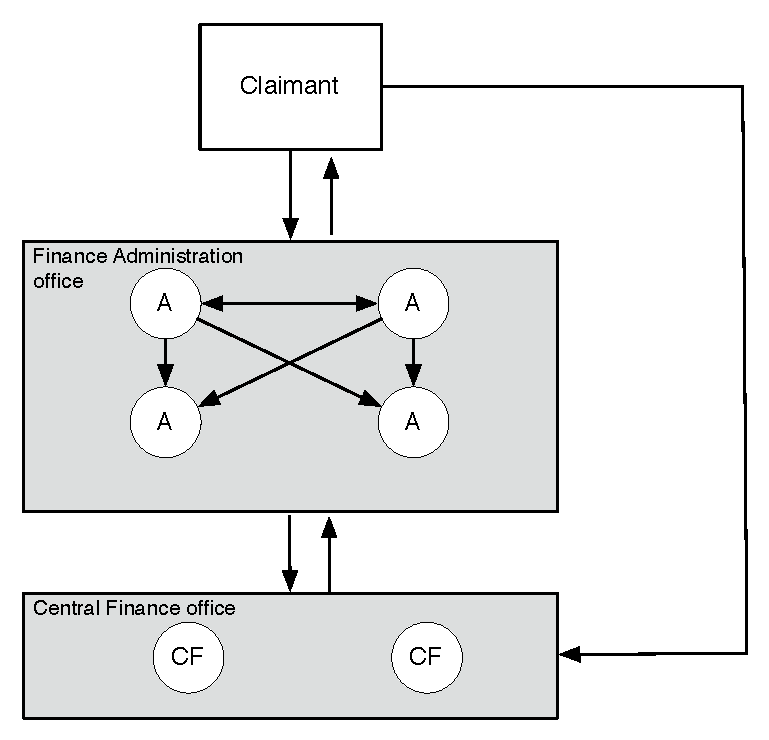
\includegraphics[width=0.3\textwidth]{images/ch12/ch12_infmodel.pdf}
\caption[Study 2 Information flow model]{Model of the information flow.}
\vspace{-9pt}
\label{fig:ch12_infmod}
\end{figure}


An expenses claim \textit{moves} through several actors, and moves between actors via email, phone, physical post, and face-to-face communication. The actors who contribute to the processing of an expense claim have limited visibility on the overall status and progress of the claim. For example, once claimants submit a claim request to the administrator, they do not know what the status is of that claim until they receive an email notification that it has been completed. Similarly, once administrators submit a claim to the Central Finance office, they do not know what the status is of the claim. They do not know when or whether it has been processed and if not, what the reasons are for holding it. The workers at the Central Finance office know the reasons for withholding a claim, but often receive incomplete information of a claim, and for example do not know the justification behind a claim, whether the expenses are made correctly and if there is an error in the project code entry, they do not know the correct project to charge it to.

\textit{Information transformation} takes place when calculations have to be carried out. At the beginning the individual numbers are saved, as well as the calculations on those numbers. Once a claim is submitted only the end result will be saved on the system. For example, if one claim request involves multiple expenses, each individual amount has to be checked by the administrator. Administrators are then free to choose whether to type each amount or only the sum total on the system. Once they have processed and submitted the claim, only the sum amount will be available for auditors. 

There are two main \textit{information hubs}: the first hub is the office of the administrator, who deals with incoming claims and hard-copy receipts from claimants. These claims are processed at the administrator office and then sent off to the Central Finance office, the second information hub. Workers at this office deal with incoming claims and hard-copy receipts from administrators, match and process these and submit them for payment. 

The administrator is the main\textit{ information buffer }between the claimant and the Central Finance officers. Claimants submit a request to administrators. This claim is upheld until the administrator decides to process it and send it to Central Finance. If there was an issue with a claim, claimants contacted the administrator, who then contacted Central Finance. Though claimants could also contact Central Finance directly, administrators said it was often easier if they contacted Central Finance on their behalf, as they knew who to contact [quote]. 

\textit{Communication} between the claimant and administrator takes place face-to-face, over the phone, via email and via handwritten notes. Communication between colleagues takes place face-to-face. Communication between the administrator and Central Finance solely takes part via email or over the phone, though it is possible to take place face-to-face.

Instructions are mostly \textit{communicated informally} through word of mouth. Knowledge of how to use the system sits with the employees, and it is often faster to explain newcomers how to do it rather than go through the written instructions. A consequence is that when information gets updated, not everyone is aware of it and keeps using the old and incorrect way, or learn the incorrect way from someone else who is still using the old way. 

Receiving a claim request from another actor are the main \textit{factors triggering behaviour.} Participants collected claim requests and saved them to return to later. Some participants kept claims to be completed on their desk. The size of this pile acted as a trigger to decide whether to start processing them. Furthermore, the payroll deadline was another trigger. Participants tried to complete claims before the deadline so claimants were reimbursed in time.

\subsubsection{Task strategies}
By describing the task environment, several strategies were uncovered. These are discussed in more detail below. After developing the models, the audio transcripts, notes, and video recordings were reviewed again to identify patterns of information strategies. 

\textbf{Planning for information needs}
Participants started processing an expense claim by collected all physical sources they knew they were going to need. These were the paper receipts, and could include a physical claim form and notes with written instructions. They placed this on a pile on their desk next to their computer, and entered this information first. 

Participants did not collect digital sources beforehand. Instead, participants retrieved these sources at the moment in the task they realised they needed it. When they realised they needed information from a digital source, they interrupted entering data, left the data entry window and went to search for the information. 

Participants did not always know beforehand what the cost of collecting this data was going to be, but assumed it could be retrieved fairly quickly. Sometimes it could take longer than expected due to various reasons. First, they did not always know which source to consult for finding the data. For example, people in Central Finance had to validate if the person signing off a claim form was authorised to give this signatory. The information to check this could be in a spreadsheet, but was sometimes also in a different PDF file. At other times, this information had to be looked up on the departmental intranet. Second, if participants did know which specific source to access, they did not always know the associated cost to access it. If information about a certain employee needed to be looked up, people consulted a search engine and typed in the person?s name. Sometimes they found the information quickly, but sometimes it took a while before they found what they needed. Third, even if participants did know the specific source and the normal cost, this cost was not always the same. For example, a website could take longer to load than usual.

If information was difficult to find, participants had time thresholds to decide whether to postpone it and come back to it later. P2 said that if he felt he was spending more than ten minutes on a task, he would postpone it. He placed uncompleted expense claims that required further attention in a separate tray on his desk. He revisited this pile the next morning and tried to process them then.
During observations, P5 could not find certain information for a claim either. After approximately five minutes of trying to find the information, she decided to write an email to the claimant requesting the information. She then put the claim form aside and started the next expenses task.
 
 \textbf{Creation of information sources}
Participants had access to shared files on the intranet of the office. They did not always find this information easy to use, and sometimes made their own local copies.
%Furthermore, collecting and organising information can be time-consuming (Bardram et al., 2006). This was also observed in the current study. 

\textbf{Deferral of interruptions}
In order to prevent people from interrupting an expenses task, people were logged out of the data entry system after a period of inactive use and they had to restart the task from the beginning. This added cost to resume the task kept participants focused on the data entry task, and they were less likely to interrupt and switch to unrelated tasks.
Participants did however interrupt a data entry task for task-related purposes, such as looking up information. They left the data entry interface and opened a new window. As windows were maximised, they were unable to see the data entry interface whilst they were looking up information. Participants explained it was much easier and faster to look up information on the screen they were already interacting with, rather than switch screens. They also felt that, opposed to physical sources, they could retrieve information from digital sources quickly. It sometimes took longer than expected however to look up certain information. Furthermore, it was also not clear how long the system would wait before logging them out. Upon coming back to the data entry interface, participants often found that they were logged out unexpectedly, needed to log back in and start from the beginning. In most cases, their information was lost.

\textbf{Use of multiple screens}
People dedicated one screen for the expenses task and maximised their window, so it filled the entire screen. This is in accordance with Bi and Balakrishnan (2009), who found that when dealing with two screens, people dedicate one computer screen to the primary task. However, they found that they use a second screen for subtasks. This was also found by Dearman and Pierce (2008)'s study on how people use multiple devices found that people assign sub-tasks to secondary devices to minimise the need to transfer information between devices.
People in the current study often also used their primary screen to look up information for the expenses task, and switched back and forth between maximised windows, rather than look up and display information on the second screen. In contrast, previous studies on the use of multiple screens showed that people dedicated a second screen to look up information \citep{Bi2009, Gurdin2001}. Even if people knew beforehand which digital information they were going to need, they often started the task and looked up information as they needed it. For paper information, they did collect all information they knew they were going to need, such as the paper receipts, the claim form, and any additional post-its with instructions. 
Whilst there was a possibility to place information on the second screen, this is also time-consuming \citep{Bardram2006}. With paper sources, it is perhaps less time-consuming: no time was spent on arranging the sources on the physical space of the desk, but they were stacked in a pile on their desk or lap and the right source was picked out when needed.
\citet{Dearman2008}'s study on how people use multiple devices found that people assign sub-tasks to secondary devices to minimise the need to transfer information between devices. Potentially people used the primary screen for looking up information so the information was on one screen and try could try to copy and paste it. Often though this was either not possible or users chose themselves to manually transcribe it.
 
People used additional screens for other tasks. For example, the second screen was often used to display the email inbox, but this was not consulted during the expenses task. Even in instances when people had to look up information from an email, they would open their inbox on the primary screen, rather than look it up on the second screen. 


\subsection{Discussion}
The purpose of this study was to investigate the information sources people need for an expenses task, and how they currently manage subtasks of looking up information from an expenses task.  Do they look up information as they need it, or get all the required information first and then enter it? Do they change their strategies as they get more experienced with the task and know where to get the information from?

The following questions were addressed:

\begin{enumerate}
\item 
What is the information needed for an expenses task?
\item 
Where is this information retrieved from?
\item 
What are the strategies people use to look up information?
\end{enumerate}

%WHAT INFORMATION AND WHERE FROM
\subsubsection{Information sources}
%Paper and digital sources
%Availability of information
The information needed for an expenses task needed to be retrieved from both paper sources, such as paper receipts, handwritten instructions and claim forms, as well as digital sources, such as spreadsheets, websites and emails.

The user did not always know beforehand what the cost of accessing digital sources was going to be. First, they did not always know which source to consult for finding the data. For example, people in Central Finance had to validate if the person signing off a claim form was authorised to give this signatory. The information to check this could be in a spreadsheet, but was sometimes also in a different PDF file. At other times, this information had to be looked up on the departmental intranet. Second, if participants did know which specific source to access, they did not always know the associated cost to access it. If information about a certain employee needed to be looked up, people consulted a search engine and typed in the person?s name. Sometimes they found the information quickly, but sometimes it took a while before they found what they needed. Third, even if participants did know the specific source and the normal cost, this cost was not always the same. For example, a website could take longer to load than usual.

Information was centrally available, but this was perceived as being difficult to use. As a result, users made their own local copies of information they needed and used these sources instead. Furthermore, procedural information was passed on via colleagues rather than the central information sources. This caused people to use outdated information. Multiple departments were involved in the task. There was no transparency of information and progress of activity, and explicit information exchange was needed. The system had a timeout to prevent long interruptions, but people still looked up information as they needed it. They often did not know the associated IAC and as a result were locked out. 

%WHAT ARE THE STRATEGIES PEOPLE USE
\subsubsection{Information strategies}
%Collect physical sources in a batch, before starting a task, %Lookup digital information as they need it 
With paper sources, no time was spent on arranging the sources on the physical space of the desk, but they were stacked in a pile on their desk or lap and the right source was picked out when needed.

People did not always know which information they were going to need for a task, which made it challenging to collect all information beforehand. Therefore, people usually started a task collecting physical sources they knew were needed, and looked up other information as they needed it. Even if people knew beforehand which digital sources they were going to need, they still looked up information as they needed it.

This is in contrast with \citet{Sohn2008}, who found that uncertainty of the location of information would cause people to leave looking for it until later. A difference with this study is that Sohn et al. (2008) looked at people?s information search behaviour for personal tasks. Perhaps there was a pressure for employees to finish their work tasks and the urgency of finishing the task weighed more than the potential time cost of looking up information.

%Use of multiple screens
People dedicated one screen for the expenses task and maximised their window, so it filled the entire screen. People in the current study often also used their primary screen to look up information for the expenses task, and switched back and forth between maximised windows, rather than look up and display information on the second screen. 

Previous studies on the use of multiple screens showed that people dedicated a second screen for subtasks that supported the main task, such as looking up information \citep{Bi2009, Dearman2008, Grudin2001}. Even if people knew beforehand which digital sources they were going to need, they often started the task without placing this on the second screen. They did not look up information until they needed it, and used their main screen for this.

Whilst there was a possibility to place information on the second screen, this is also time-consuming \citep{Bardram2006}. 
\citet{Dearman}'s study on how people use multiple devices found that people assign sub-tasks to secondary devices to minimise the need to transfer information between devices. Potentially people used the primary screen for looking up information so the information was on one screen and try could try to copy and paste it. Often though this was either not possible or users chose themselves to manually transcribe it.
 
People used additional screens for other tasks. For example, the second screen was often used to display the email inbox, but this was not consulted during the expenses task. Even in instances when people had to look up information from an email, they would open their inbox on the primary screen, rather than look it up on the second screen. This contrasts \citep{Grudin2001} where people deliberately used a second screen to look up information, even if it was  faster to retrieve it from their primary screen.

%Use of local copies

\subsubsection{Other issues}

\subsubsection{Contribution}
\begin{itemize}
\item
Evidence that an expenses task is fragmented: people often have to go in and out of the expenses system to look up information.    
\item
Evidence that the IAC of the required information sources for an expenses task varies. 
\item
Evidence that depending on people's experience and awareness of how costly it is to access information, they will try to minimise switching between tasks.
\end{itemize}

The goal of this study was to give an understanding of how people manage subtasks of looking up information as part of data entry work in a financial office.

\subsubsection{Limitations}
The goal of this study was to get an understanding of how people collect information as part of data entry work in a financial office. By using a Distributed Cognition approach, it became clear that information for an expenses task was not only distributed between external artefacts and internal cognition of one individual, but also between people. 
As the focus of analysis of this study was on the individual and not the team, the human agents are included as additional information sources. Studying distribution of cognition from a teamwork point of view is beyond the scope of this thesis, but will be useful to study in future work. Several issues became clear that related to teamwork, such as limitations in communication and coordination of central information. 

Due to confidentiality issues surrounding financial data, it was not possible to install logging software on participants' computers and all observational data reported here is qualitative. 
Given the situated nature of the study, it is also not clear to what extent people's behaviour is shaped by the access of the information sources, and how they are influenced by other situational factors such as user expertise. 
The next series of studies are set in a controlled environment, with the aim to study the influence of access costs to information on people's strategies, and how strategies impact quantitative performance measures as accuracy and speed. Study 1 and 2 have given an understanding of the task context and the information sources. The materials used in the subsequent studies will be designed to look similar to the office setting.
